\section{正交变换与直角坐标变换}

正交变换是一种线性变换, 它保持向量的内积不变, 即在变换前后, 向量的模长和夹角保持不变. 这种变换可以通过正交矩阵来实现, 这些矩阵的特征值的绝对值为 1, 并且可以准对角化. 在图形学中, 正交变换可以用来调整图形, 使其更加规整而不改变其大小和形状.

直角坐标变换则是指在平面上, 从一个直角坐标系到另一个直角坐标系的坐标转换, 这种转换通常涉及到坐标轴的旋转或平移. 正交变换与直角坐标变换不同, 因为它不仅仅是坐标的简单转换, 而是在保持向量内积不变的同时进行坐标系的变换.

\subsection{正交变换}

\begin{definition}[正交矩阵]
    设 $\vb*{A}$ 为 $n$ 阶实对称矩阵, 则存在正交矩阵 $\vb*{Q}$, 使得
    $$\vb*{Q}^{-1}\vb*{AQ}=\vb*{Q}^\top\vb*{AQ}=\mqty(\dmat{\lambda_1,\lambda_2,\ddots,\lambda_n})$$
    其中 $\lambda_1,\lambda_2,\cdots,\lambda_n$ 是 $\vb*{A}$ 的特征值, 矩阵 $\vb*{Q}$ 的列向量是对应的正交规范化的特征向量.
\end{definition}

\begin{theorem}[正交变换与相似]
    若二次型 $\vb*{x}^\top\vb*{Ax}$ 经正交变换 $\vb*{x}=\vb*{Qy}$ 有 $\vb*{x}^\top\vb*{Ax}=\vb*{y}^\top\vb*{By}$, 则 $\vb*{A}\sim\vb*{B}.$
\end{theorem}

\begin{theorem}[正交矩阵的行列式]
    若方阵 $\vb*{A}$ 是正交矩阵, 那么等价为 实方阵 $\vb*{A}$ 的行列式等于 $\pm1$, 并且当 $|\vb*{A}|=1$ 时, $\vb*{A}$ 的每一个元素等于该元素的代数余子式, 即 $a_{ij}=A_{ij}$;
    当 $|\vb*{A}|=-1$ 时, $\vb*{A}$ 的每一个元素等于该元素的代数余子式乘以 $-1$, 即 $a_{ij}=-A_{ij}.$
\end{theorem}
\begin{proof}[{\songti \textbf{证}}]
    \textbf{充分性: }设 $\vb*{A}$ 是正交矩阵, 则 $\vb*{AA}^\top=\vb*{E}$, 所以 $|\vb*{A}|^2=1$, 即 $|\vb*{A}|=\pm1$, 若 $|\vb*{A}|=1$, 则 $\vb*{A}^*=|\vb*{A}|\vb*{A}^{-1}=\vb*{A}^\top$, 比较等式两边对应的元素, 得 $a_{ij}=A_{ij}~~(1\leqslant i,j\leqslant n)$;
    同理当 $|\vb*{A}|=-1$, 可证 $a_{ij}=-A_{ij}$, \\
    \textbf{必要性: }当 $|\vb*{A}|=1$ 时, 由 $a_{ij}=A_{ij}~~(1\leqslant i,j\leqslant n)$, 有 $\vb*{A}^{-1}=\dfrac{1}{|\vb*{A}|}\vb*{A}^*=\vb*{A}^\top$; 当 $|\vb*{A}|=-1$ 时, 由 $a_{ij}=-A_{ij}~~(1\leqslant i,j\leqslant n)$, 有 $\vb*{A}^{-1}=\dfrac{1}{|\vb*{A}|}=-(-\vb*{A})^\top=\vb*{A}^\top$, 所以 $\vb*{A}$ 是正交矩阵.
\end{proof}

\begin{example}
    求例题 \ref{fx1x2x3gy1y2y3} 中, 是否存在正交变换 $\vb*{x}=\vb*{Q}\vb*{y}$ 将 $f$ 化为 $g.$
\end{example}
\begin{solution}
    二次型 $f$ 对应的矩阵为 $\vb*{A}=\mqty(1&1&-1\\1&2&0\\-1&0&2)$, 其特征方程为 $$|\lambda\vb*{E}-\vb*{A}|=\mqty|\lambda-1&-1&1\\-1&\lambda-2&0\\1&0&\lambda-2|=\lambda(\lambda-2)(\lambda-3)=0$$
    则 $\lambda_1=0,\lambda_2=2,\lambda_3=3$, 同理可得 $g$ 的特征值为 $0,1,2$, 因为特征值不全相等, 故 $\vb*{A}\not\sim \vb*{B}$, 因此不存在正交矩阵 $\vb*{Q}$ 使得在正交变换 $\vb*{x}=\vb*{Q}\vb*{y}$ 下将 $f$ 化为 $g.$
\end{solution}

\begin{example}
    已知二次型 $f(x_1,x_2,x_3)=2x_1^2+ax_3^2+2x_2x_3$ 经正交变换 $\vb*{x}=\vb*{Py}$ 可化为标准形 $y_1^2+by_2^2-y_3^2$, 求 $a+b.$
\end{example}
\begin{solution}
    由题意 $\vb*{A}=\mqty(2&0&0\\0&0&1\\0&1&a),~\vb*{B}=\mqty(\dmat{1,b,-1})$, 且 $\vb*{A}\sim\vb*{B}$, 则
    $$\begin{cases}
            \tr\vb*{A}=\tr\vb*{B}   \\
            \det\vb*{A}=\det\vb*{B} \\
        \end{cases}\Rightarrow\begin{cases}
            2+a=b \\-2=-b
        \end{cases}\Rightarrow a+b=2.$$
\end{solution}

\begin{example}
    设 $\vb*{\alpha},~\vb*{\beta}$ 是三维列向量, 且 $[\vb*{\alpha},\vb*{\beta}]=-1$, 又 $\vb*{A}=\vb*{E}-\vb*{\alpha\beta}^\top$ 求 $(\vb*{A}+\vb*{E})^{-1}.$
\end{example}
\begin{solution}
    因为 $[\vb*{\alpha},\vb*{\beta}]=-1$ (两个向量的内积), 所以
    $$\vb*{A}^2=\qty(\vb*{E}-\vb*{\alpha\beta}^\top)\qty(\vb*{E}-\vb*{\alpha\beta}^\top)=\vb*{E}-2\vb*{\alpha\beta}^\top+\vb*{\alpha}\underbrace{\vb*{\beta}^\top\cdot\vb*{\alpha}}_{[\vb*{\alpha},\vb*{\beta}=-1]}\vb*{\beta}^\top=\vb*{E}-3\vb*{\alpha\beta}^\top=3\qty(\vb*{E}-\vb*{\alpha\beta}^\top)-2\vb*{E}=3\vb*{A}-2\vb*{E}$$
    即 $\vb*{A}^2-3\vb*{A}+2\vb*{E}=\vb*{O}\Rightarrow (\vb*{A}+\vb*{E})(\vb*{A}-4\vb*{E})+6\vb*{E}=\vb*{O}\Rightarrow (\vb*{A}+\vb*{E})\dfrac{\vb*{A}-4\vb*{E}}{-6}=\vb*{E}\Rightarrow (\vb*{A}+\vb*{E})^{-1}=\dfrac{4\vb*{E}-\vb*{A}}{6}.$
\end{solution}

% \begin{example}
%     已知二次型 $$f(x_1,x_2,x_3)=\vb*{x}^\top\vb*{Ax}=ax_1^2+ax_2^2+ax_3^2+2x_1x_2+2x_1x_3-2x_2x_3$$ 的标准形为 $y_1^2+y_2^2$, 
%     \begin{enumerate}[label=(\arabic{*})]
%         \item 求 $a$ 的值;
%         \item 利用正交变换将二次型 $f$ 化为标准形, 并写出所用的正交变换.
%     \end{enumerate}
% \end{example}
% \begin{solution}
%     \begin{enumerate}[label=(\arabic{*})]
%         \item 
%     \end{enumerate}
% \end{solution}

\begin{example}
    设 $\vb*{\alpha},\vb*{\beta}$ 均为 3 维单位列向量, $\vb*{\alpha}^\top\vb*{\beta}=\dfrac{1}{2},~\vb*{A}=\vb*{\alpha\beta}^\top+\vb*{\beta\alpha}^\top$, 求正交变换下, 二次型 $\vb*{x}^\top\vb*{Ax}$ 的标准形.
\end{example}
\begin{solution}
    先证明 $\vb*{A}$ 是实对称矩阵,
    $$\vb*{A}^\top=\qty(\vb*{\alpha\beta}^\top+\vb*{\beta\alpha}^\top)^\top=\qty(\vb*{\alpha\beta}^\top)^\top+\qty(\beta\alpha^\top)^\top=\vb*{\beta\alpha}^\top+\vb*{\alpha\beta}^\top=\vb*{A}$$
    对 $\vb*{A}$ 右乘 $\vb*{\alpha}$ 和 $\vb*{\beta}$ 得
    $$\begin{cases}
            \vb*{A\alpha}=\vb*{\alpha\beta}^\top\vb*{\alpha}+\vb*{\beta\alpha}^\top\vb*{\alpha} \\
            \vb*{A\beta}=\vb*{\alpha\beta}^\top\vb*{\beta}+\vb*{\beta\alpha}^\top\vb*{\beta}
        \end{cases}\Rightarrow\begin{cases}
            \vb*{A}(\vb*{\alpha}+\vb*{\beta})=\dfrac{3}{2}(\vb*{\alpha}+\vb*{\beta}) \\[6pt]
            \vb*{A}(\vb*{\alpha}-\vb*{\beta})=-\dfrac{1}{2}(\vb*{\alpha}-\vb*{\beta})
        \end{cases}$$
    因为 $\vb*{\alpha}^\top\vb*{\beta}=\dfrac{1}{2}\Rightarrow\vb*{\beta}^\top\vb*{\alpha}=\dfrac{1}{2}$, 且 $\vb*{\alpha}^\top\vb*{\alpha}=\vb*{\beta}^\top\vb*{\beta}=1$, 则得特征值
    $\lambda_1=\dfrac{3}{2},\lambda_2=-\dfrac{1}{2}$, 设 $\vb*{\alpha}=(a_1,a_2,a_3)^\top,~\vb*{\beta}=(b_1,b_2,b_3)^\top$,
    那么 $$\tr\vb*{A}=2a_1b_1+2a_2b_2+2a_3b_3=2\vb*{\alpha}^\top\vb*{\beta}=1\Rightarrow \lambda_3=\tr\vb*{A}-\lambda_1-\lambda_2=0$$
    于是 $\vb*{x}^\top\vb*{Ax}$ 的标准形为 $\dfrac{3}{2}y_1^2-\dfrac{1}{2}y_2^2.$
\end{solution}

\begin{example}
    设二次型 $f(x_1,x_2,x_3)=(x_1-2x_2)^2+(x_2-x_3)^2+(x_1+ax_3)^2$,
    \begin{enumerate}[label=(\arabic{*})]
        \item 求 $f(x_1, x_2, x_3)=0$ 的解;
        \item 设二次型 $f(x_1, x_2, x_3)$ 的规范形为 $z_1^2, z_2^2$, 求正交变换 $\vb*{x}=\vb*{Qy}$, 使得二次型 $f(x_1, x_2, x_3)$ 化为标准形.
    \end{enumerate}
\end{example}
\begin{solution}

\end{solution}

\begin{example}
    设 3 阶实对称矩阵 $\vb*{A}$ 的秩为 2, $\lambda_1= \lambda_2=6$ 是 $\vb*{A}$ 的二重特征值, 若 $\vb*{\alpha}_1=(1,a,0)^\top,\vb*{\alpha}_2=(2,1,1)^\top,\vb*{\alpha}_3=(0,1,-1)^\top$ 都是矩阵 $\vb*{A}$ 属于特征值 6 的特征向量,
    \begin{enumerate}[label=(\arabic{*})]
        \item 求 $a$ 的值;
        \item 求 $\vb*{A}$ 的另一特征值和对应的特征向量;
        \item 若 $\vb*{\beta}=(-2,2,-1)^\top$, 求 $\vb*{A}^{n}\vb*{\beta}$.
    \end{enumerate}
\end{example}
\begin{solution}
    \begin{enumerate}[label=(\arabic{*})]
        \item 对于实对称矩阵 $\vb*{A}$, 若 $\lambda$ 是矩阵 $\vb*{A}$ 的 $k$ 重特征值, 则矩阵 $\vb*{A}$ 属于特征值 $\lambda$ 的特征向量有且仅有 $k$ 个是线性无关的, 因此 $\vb*{\alpha}_1, \vb*{\alpha}_2, \vb*{\alpha}_3$ 必线性相关, 那么
              $$
                  |\vb*{\alpha}_1, \vb*{\alpha}_2, \vb*{\alpha}_3|=\mqty|1 & 2 & 0 \\ a & 1 & 1 \\ 0 & 1 & -1|=2a-2=0\Rightarrow a=1.
              $$
        \item 由 $\rank\vb*{A}=2$ 知 $\det\vb*{A}=0$, 又 $\det\vb*{A}=\prod \lambda_i=0\Rightarrow \lambda_3=0$, 不同的特征值对应的特征向量相互正交, 则 $\vb*{\alpha}_2\times\vb*{\alpha}_3=(-2,2,2)$, 那么矩阵 $\vb*{A}$ 属于特征值 $\lambda_3=0$ 的全部特征向量为 $k\vb*{\alpha}=k(-1,1,1)^\top.$
        \item 设 $x_1\vb*{\alpha}_1, x_2\vb*{\alpha}_2, x_3\vb*{\alpha}=\vb*{\beta}$, 对 $\begin{pNiceArray}{ccc:c}\vb*{\alpha}_1&\vb*{\alpha}_2&\vb*{\alpha}_3&\vb*{\beta}\end{pNiceArray}$ 作初等行变换, 有
              $$
                  \begin{pNiceArray}{ccc:c}1 & 2 & -1 &-2\\ 1 & 1 & 1 &2\\ 0 & 1 & 1 &-1\end{pNiceArray}\xrightarrow{r_2-r_1}
                  \begin{pNiceArray}{ccc:c}1 & 2 & -1 &-2\\ 0 & -1 & 2 &4\\ 0 & 1 & 1 &-1\end{pNiceArray}\xrightarrow[r_2\times(-1)]{r_3+r_2}
                  \begin{pNiceArray}{ccc:c}1 & 2 & -1 &-2\\ 0 & 1 & -2 &-4\\ 0 & 0 & 3 &3\end{pNiceArray}
              $$
              解得 $x_1=3, x_2=-2, x_3=1$, 故 $\vb*{\beta}=3\vb*{\alpha}_1-2\vb*{\alpha}_2+\vb*{\alpha}$, 因为 $\vb*{A\alpha}_1=6\vb*{\alpha}_1, \vb*{A\alpha}_2=6\vb*{\alpha}_2, \vb*{A\alpha}=0\vb*{\alpha}$, 所以
              $$\vb*{A}^{n}\vb*{\beta}=3\vb*{A}^{n}\vb*{\alpha}_1-2\vb*{A}^{n}\vb*{\alpha}_2+\vb*{A}^{n}\vb*{\alpha}=3\cdot 6^{n}\vb*{\alpha}_1-2\cdot 6^{n}\vb*{\alpha}_2=\qty(-6^{n},6^{n},-2\cdot 6^{n})^{\top}.$$
    \end{enumerate}
\end{solution}

\begin{example}
    若二次型 $f(x_1, x_2, x_3)=x_1^2+2x_2^2+x_3^2-2x_1x_3$, 经正交变换 $\vb*{x}=\vb*{Qy}$ 化为二次型 $g(y_1, y_2, y_3)=y_1^2+y_2^2+ay_3^2+2y_1y_2$, 求 $a$ 与矩阵 $\vb*{Q}$.
\end{example}
\begin{solution}
    由题意知 $\vb*{A}=\begin{pmatrix} 1 & 0 & -1 \\ 0 & 2 & 0 \\ -1 & 0 & 1 \\\end{pmatrix}, \vb*{B}=\begin{pmatrix} 1 & 1 & 0 \\ 1 & 1 & 0 \\ 0 & 0 & a \\\end{pmatrix}$, 且 $\vb*{A}\sim \vb*{B}$, 于是 $\tr\vb*{A}=\tr\vb*{B}\Rightarrow a=2$, 又
    $$
        |\lambda\vb*{E}-\vb*{A}|=\mqty|\lambda-1 & 0 & 1 \\ 0 & \lambda-2 & 0 \\ 1 & 0 & \lambda-1 |=\lambda(\lambda-2)^2=0\Rightarrow \lambda_1=0,\lambda_2=\lambda_3=2
    $$
    当 $\lambda=\lambda_1=0$ 时, 对应的特征向量为 $\vb*{\xi}_1=\mqty(1\\0\\1)$, 当 $\lambda=\lambda_{2,3}=2$ 时, 对应的特征向量分别为
    $\vb*{\xi}_2=\mqty(1\\0\\-1),\vb*{\xi}_3=\mqty(0\\1\\0)$, 令 $\vb*{Q}_1=\qty(\dfrac{\vb*{\xi}_1}{\norm*{\vb*{\xi}_1}},\dfrac{\vb*{\xi}_2}{\norm*{\vb*{\xi}_2}},\dfrac{\vb*{\xi}_3}{\norm*{\vb*{\xi}_3}})=\mqty(\dfrac{1}{\sqrt{2}}&\dfrac{1}{\sqrt{2}}&0\\ 0&0&1\\ \dfrac{1}{\sqrt{2}}&-\dfrac{1}{\sqrt{2}}&0)$, 二次型 $f(\vb*{x})$ 在 $\vb*{x}=\vb*{Q}_1\vb*{z}$ 下化为 $f(\vb*{z})=z_2^2+z_3^2$, 同样的, 当 $\lambda=\lambda_1=0$ 时, 对应的特征向量为 $\vb*{\eta}_1=\mqty(1\\-1\\0)$, 当 $\lambda=\lambda_{2,3}=2$ 时, 对应的特征向量分别为 $\vb*{\eta}_2=\mqty(1\\1\\0),\vb*{\xi}_3=\mqty(0\\0\\1)$, 令 $\vb*{Q}_2=\qty(\dfrac{\vb*{\eta}_1}{\norm*{\vb*{\eta}_1}},\dfrac{\vb*{\eta}_2}{\norm*{\vb*{\eta}_2}},\dfrac{\vb*{\eta}_3}{\norm*{\vb*{\eta}_3}})=\mqty(\dfrac{1}{\sqrt{2}}&\dfrac{1}{\sqrt{2}}&0\\[6pt]-\dfrac{1}{\sqrt{2}}&\dfrac{1}{\sqrt{2}}&0\\0&0&1)$, 二次型 $g(\vb*{y})$ 在 $\vb*{y}=\vb*{Q}_2\vb*{z}$ 下化为 $g(\vb*{y})=z_2^2+z_3^2$, 则
    $$\vb*{Q}=\vb*{Q}_1\vb*{Q}_2^{-1}=\vb*{Q}_1\vb*{Q}_2^\top=\begin{pmatrix} 1 & 0 & 0 \\ 0 & 0 & 1 \\ 0 & -1 & 0 \\\end{pmatrix}.$$
\end{solution}

\begin{example}
    已知 $\vb*{A}=\mqty(0&1&1&-1\\1&0&-1&1\\1&-1&0&1\\-1&1&1&0)$,
    求正交矩阵 $\vb*{P}$, 使 $\vb*{P}^\top\vb*{AP}$ 成为对角矩阵.
\end{example}
\begin{solution}
    特征多项式 $f(\lambda)$ 为:
    \begin{flalign*}
        f(\lambda) & =|\lambda\vb*{E}-\vb*{A}|=\mqty|\lambda                                        & -1  & -1  & 1 \\-1&\lambda&1&-1\\-1&1&\lambda&-1\\1&-1&-1&\lambda|\xlongequal[r_3+r_4]{\substack{r_1-r_4\\r_2+r_4}}\mqty|\lambda-1&0&0&1-\lambda\\0&\lambda-1&0&\lambda-1\\0&0&\lambda-1&\lambda-1\\1&-1&-1&\lambda|\\
                   & =\sum_{1\leqslant i_1<i_2<i_3\leqslant 4}\vb*{A}\mqty(i_1                      & i_2 & i_3     \\1&2&3)\qty[(-1)^{i_1+i_2+i_3+1+2+3}\vb*{A}\mqty(i_4\\4)]\\
                   & =\lambda\mqty|\dmat{\lambda-1,\lambda-1,\lambda-1}|-(\lambda-1)\mqty|\lambda-1 & 0   & 0       \\0&\lambda-1&0\\1&-1&1|+(\lambda-1)\mqty|\lambda-1&0&0\\0&0&\lambda-1\\1&-1&-1|\\
                   & =(\lambda-1)^3(\lambda+3)=0
    \end{flalign*}
    解得 $\vb*{A}$ 的特征值为 $\lambda_1=1$ (三重), $\lambda_2=-3$, 对于 $\lambda_1=1$, 可求得 $\vb*{A}$ 的相应的 3 个线性无关的特征向量为
    $$\vb*{\alpha}_1=(1,1,0,0)^\top,~\vb*{\alpha}_2=(1,0,1,0)^\top,~\vb*{\alpha}_3=(-1,0,0,1)^\top$$
    利用 Schmidt 正交化方法, 得
    $$\vb*{\xi}_1=\dfrac{1}{\sqrt{2}}(1,1,0,0)^\top,~\vb*{\xi}_2=\dfrac{1}{\sqrt{6}}(1,-1,2,0)^\top,~\vb*{\xi}_3=\dfrac{1}{\sqrt{12}}(-1,1,1,3)^\top$$
    对于 $\lambda_2=-3$, 可求得 $\vb*{A}$ 的相应的一个线性无关的特征向量为 $\vb*{\alpha}_4=(1,-1,-1,1)^\top$, 把它单位化得 $\vb*{\xi}_4=\dfrac{1}{2}(1,-1,-1,1)^\top$,
    于是有 $\vb*{P}^\top\vb*{AP}=\mathrm{diag}(1,1,1,-3)$, 其中正交矩阵 $\vb*{P}$ 为
    $$\vb*{P}=\qty(\vb*{\xi}_1,\vb*{\xi}_2,\vb*{\xi}_3,\vb*{\xi}_4)=\mqty(\dfrac{1}{\sqrt{2}}&\dfrac{1}{\sqrt{6}}&-\dfrac{1}{\sqrt{12}}&\dfrac{1}{2}\\[6pt]\dfrac{1}{\sqrt{2}}&-\dfrac{1}{\sqrt{6}}&\dfrac{1}{\sqrt{12}}&-\dfrac{1}{2}\\[6pt]0&\dfrac{2}{\sqrt{6}}&\dfrac{1}{\sqrt{12}}&-\dfrac{1}{2}\\[6pt]0&0&\dfrac{3}{\sqrt{12}}&\dfrac{1}{2}).$$
\end{solution}

\begin{example}[2010 武汉大学]
    设三阶实对称矩阵 $\vb*{A}$ 的各行元素之和均为 3, 向量
    $$\vb*{\alpha}_1=(-1,2,-1)^{\top},~\vb*{\alpha}_2=(0,-1,1)^{\top}$$ 是线性方程组 $\vb*{Ax}=\vb*{0}$ 的两个解.
    \begin{enumerate}[label=(\arabic{*})]
        \item 求 $\vb*{A}$ 的特征值与特征向量;
        \item 求正交矩阵 $\vb*{Q}$ 和对角矩阵 $\vb*{D}$, 使得 $\vb*{Q}^{\top}\vb*{AQ}=\vb*{D}$;
        \item 求行列式 $\qty|\qty(\dfrac{2}{3}\vb*{B}^2)^{-1}+\dfrac{4}{9}\vb*{B}^*+\vb*{B}|$, 其中 $\vb*{B}$ 是 $\vb*{A}-\dfrac{3}{2}\vb*{E}$ 的相似矩阵, $\vb*{B}^*$ 为 $\vb*{B}$ 的伴随矩阵.
    \end{enumerate}
\end{example}
\begin{solution}
    \begin{enumerate}[label=(\arabic{*})]
        \item 因为 $\vb*{A\alpha}_1=\vb*{0}=0\vb*{\alpha}_1,~\vb*{A\alpha}_2=\vb*{0}=0\vb*{\alpha}_2$, 所以 $\lambda_1=\lambda_2=0$ 是 $\vb*{A}$ 的二重特征值, $\vb*{\alpha}_1,~\vb*{\alpha}_2$ 是 $\vb*{A}$ 的属于特征值
              0 的两个线性无关的特征向量; 又 $\vb*{A}$ 的各行元素之和均为 3, 所以 $$\vb*{A}(1,1,1)^{\top}=(3,3,3)^{\top}=3(1,1,1)^{\top}$$
              则 $\lambda_3=3$ 是 $\vb*{A}$ 的一个特征值, $\vb*{\alpha}_3=(1,1,1)^{\top}$ 是 $\vb*{A}$ 的属于特征值 3 的特征向量, 总之, $\vb*{A}$ 的特征值为 $0,0,3$, 属于特征值 0 的所有特征向量为 $k_1\vb*{\alpha}_1+k_2\vb*{\alpha}_2$ ($k_1,~k_2\text{ 不全为零}$),
              属于特征值 3 的所有特征向量为 $k_3\vb*{\alpha}_3~  (k_3\neq0)$.
        \item 先将 $\vb*{\alpha}_1,~\vb*{\alpha}_2$ 正交化 $$\vb*{\xi}_1=\vb*{\alpha}_1=(-1,2,-1)^{\top},~\vb*{\xi}_2=\vb*{\alpha}_2-\dfrac{\comm{\vb*{\alpha}_2}{\vb*{\xi}_1}}{\norm*{\vb*{\xi}_1}^2}\vb*{\xi}_1=\qty(-\dfrac{1}{2},0,\dfrac{1}{2})^{\top}$$
              再将 $\vb*{\xi}_1,~\vb*{\xi}_2,~\vb*{\alpha}_3$ 单位化, 得
              \begin{flalign*}
                  \vb*{e}_1=\dfrac{\vb*{\xi}_1}{\norm*{\vb*{\xi}_1}}=\dfrac{1}{\sqrt{6}}(-1,2,-1)^{\top},~\vb*{e}_2=\dfrac{\vb*{\xi}_2}{\norm*{\vb*{\xi}_2}}=\dfrac{1}{\sqrt{2}}(-1,0,1)^{\top},~\vb*{e}_3=\dfrac{\vb*{\alpha}_3}{\norm*{\vb*{\alpha}_3}}=\dfrac{1}{\sqrt{3}}(1,1,1)^{\top}
              \end{flalign*}
              那么 $\vb*{Q}=(\vb*{e}_1,\vb*{e}_2,\vb*{e}_3)=\mqty(-\dfrac{1}{\sqrt{6}} &-\dfrac{1}{\sqrt{2}} &\dfrac{1}{\sqrt{3}}\\[6pt] \dfrac{2}{\sqrt{6}} &0 &\dfrac{1}{\sqrt{3}}\\[6pt] -\dfrac{1}{\sqrt{6}} &\dfrac{1}{\sqrt{2}} &\dfrac{1}{\sqrt{3}})$
              于是 $\vb*{D}=\mqty(\dmat{0,0,3})$.
        \item 因为 $\vb*{B}$ 相似于 $\vb*{A}-\dfrac{3}{2}\vb*{E}$, 而 $\vb*{A}-\dfrac{3}{2}\vb*{E}$ 相似于 $\vb*{D}-\dfrac{3}{2}\vb*{E}$, 于是 $\vb*{B}$ 相似于 $\vb*{D}-\dfrac{3}{2}\vb*{E}$, 故
              $$|\vb*{B}|=\qty|\vb*{D}-\dfrac{3}{2}\vb*{E}|=\qty(\dfrac{3}{2})^3=\dfrac{27}{8}\Rightarrow \vb*{B}^*=|\vb*{B}|\cdot \vb*{B}^{-1}$$
              \begin{flalign*}
                  \qty(\dfrac{2}{3}\vb*{B}^2)^{-1}+\dfrac{4}{9}\vb*{B}^*+\vb*{B}=\vb*{B}\qty(\dfrac{3}{2}\qty(\vb*{B}^{-1})^3+\dfrac{3}{2}\qty(\vb*{B}^{-1})^2+\vb*{E})=\vb*{B}\varphi\qty(\vb*{B}^{-1})
              \end{flalign*}
              其中 $\varphi(x)=\dfrac{3}{2}x^3+\dfrac{3}{2}x^2+1$, 因为 $\vb*{B}^{-1}$ 的特征值为 $-\dfrac{2}{3},~-\dfrac{2}{3},~\dfrac{2}{3}$, 所以 $\varphi\qty(\vb*{B}^{-1})$ 特征值为
              \begin{flalign*}
                  \varphi\qty(-\dfrac{2}{3})=\dfrac{3}{2}\qty(-\dfrac{2}{3})^3+\dfrac{3}{2}\qty(-\dfrac{2}{3})^2+1=\dfrac{11}{9}~  \text{(二重) } \varphi\qty(\dfrac{2}{3})=\dfrac{3}{2}\qty(\dfrac{2}{3})^3+\dfrac{3}{2}\qty(\dfrac{2}{3})^2+1=\dfrac{19}{9}
              \end{flalign*}
              故所求的行列式的值为 $|d|=|\vb*{B}| \qty|\varphi\qty(\vb*{B}^{-1})|=\dfrac{27}{8}\times\qty(\dfrac{11}{9})^2\times\dfrac{19}{9}=\dfrac{2299}{216}.$
    \end{enumerate}
\end{solution}

\begin{example}
    设 $\vb*{A}$ 是 3 阶实对称矩阵, $\vb*{\alpha}=(0,-1,1)^\top,~\vb*{\beta}=(1,0,-1)^\top,~\vb*{A\alpha}=3\vb*{\beta},~\vb*{A\beta}=3\vb*{\alpha}$, 且存在 3 阶矩阵 $\vb*{B}$, 有 $\rank(\vb*{AB})<\rank\vb*{B}$,
    \begin{enumerate}[label=(\arabic{*})]
        \item 求正交变换 $\vb*{x}=\vb*{Qy}$, 化二次型 $\vb*{x}^\top\qty(\vb*{A}+\vb*{A}^*)\vb*{x}$ 为标准形, 并写出该标准形;
        \item 若 $\vb*{\gamma}=(2,0,-1)^\top$, 求 $\vb*{A}^n\vb*{\gamma}.$
    \end{enumerate}
\end{example}
\begin{solution}
    \begin{enumerate}[label=(\arabic{*})]
        \item 由 $\vb*{A\alpha}=3\vb*{\beta},~\vb*{A\beta}=3\vb*{\alpha}$, 可得 $\begin{cases}
                      \vb*{A}(\vb*{\alpha}+\vb*{\beta})=3(\vb*{\alpha}+\vb*{\beta}) \\
                      \vb*{A}(\vb*{\alpha}-\vb*{\beta})=-3(\vb*{\alpha}-\vb*{\beta})
                  \end{cases}$ 即特征值 $\lambda_1=3,~\lambda_2=-3$, 其对应的特征向量为 $$\vb*{\xi}_1=\vb*{\alpha}+\vb*{\beta}=(1,-1,0)^\top,~\vb*{\xi}_2=\vb*{\alpha}-\vb*{\beta}=(-1,-1,2)^\top$$
              因为 $\rank(\vb*{AB})<\rank\vb*{B}$, 可知 $\vb*{A}$ 不可逆, 即 $\det\vb*{A}=0$, 又 $\det\vb*{A}=\displaystyle\prod_{i=1}^{3}\lambda_i$, 故 $\lambda_3=0$, 并且 $\vb*{A}$ 是实对称矩阵, 则其特征向量相互正交, 即
              $$(1,-1,0)\times(-1,-1,2)=(-2,-2,-2)\Rightarrow (1,1,1)\Rightarrow \vb*{\xi}_3=(1,1,1)^\top$$
              则 $\vb*{A}^*$ 的特征值为\footnote{因为 $\vb*{A}^*$ 的特征值为 $\dfrac{\det\vb*{A}}{\lambda}$, 且 $\det\vb*{A}=\displaystyle\prod_{i=1}^{n}\lambda_i$, 或者可理解为 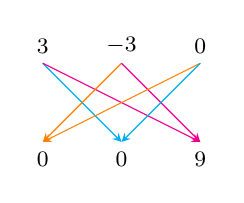
\begin{tikzpicture}[->,samples=100,>=stealth,font=\footnotesize]
                      \node[above] at (0,0) {$3$};
                      \node[above] at (1,0) {$-3$};
                      \node[above] at (2,0) {$0$};
                      \node[below] at (0,-1) {$0$};
                      \node[below] at (1,-1) {$0$};
                      \node[below] at (2,-1) {$9$};
                      \draw[cyan] (0,0)--(1,-1);
                      \draw[magenta] (0,0)--(2,-1);
                      \draw[orange] (1,0)--(0,-1);
                      \draw[magenta] (1,0)--(2,-1);
                      \draw[orange] (2,0)--(0,-1);
                      \draw[cyan] (2,0)--(1,-1);
                  \end{tikzpicture}} $\lambda_1^*=\lambda_2\lambda_3=0,~\lambda_2^*=\lambda_1\lambda_3=0,~\lambda_3^*=\lambda_1\lambda_2=-9$, 由 $\vb*{Q}^\top\vb*{AO}=\vb*{\Lambda}$ 可得
              \begin{flalign*}
                  \vb*{Q}^\top\vb*{A}^*\vb*{Q} & =\vb*{Q}^\top\qty(\vb*{Q\Lambda Q}^\top)^*\vb*{Q}=\vb*{Q}^\top\qty(\vb*{Q}^\top)^*\vb*{\Lambda}^*\vb*{Q}^*\vb*{Q}=\vb*{Q}^\top\qty|\vb*{Q}^\top|\qty(\vb*{Q}^\top)^{-1}\vb*{\Lambda}^*\qty|\vb*{Q}|\vb*{E} \\
                                               & =\vb*{Q}^\top\vb*{Q}|\vb*{Q}|\vb*{\Lambda}^*|\vb*{Q}|\vb*{E}=|\vb*{Q}|^2\vb*{\Lambda}^*\xlongequal{\det\vb*{Q}=\pm1}\vb*{\Lambda}^*
              \end{flalign*}
              因此 $\vb*{Q}^\top\qty(\vb*{A}+\vb*{A}^*)\vb*{Q}=\qty[\mqty(\dmat{3,-3,0})+\mqty(\dmat{0,0,-9})]=\mqty(\dmat{3,-3,-9})$ 即在正交变换 $\vb*{x}=\vb*{Qy}$ 下, 二次型的标准形为 $3y_1^2-3y_2^2-9y_3^2.$
        \item $\vb*{\gamma}$ 可由 $\vb*{\xi}_{1,2,3}$ 线性表示, 即 $\exists k_1,k_2,k_3$, 使得 $\vb*{\gamma}=k_1\vb*{\xi}_1+k_2\vb*{\xi}_2+k_3\vb*{\xi}_3$, 即
              $$\vb*{A}^n\vb*{\gamma}=\vb*{A}^n\qty(k_1\vb*{\xi}_1+k_2\vb*{\xi}_2+k_3\vb*{\xi}_3)=k_1\vb*{A}^n\vb*{\xi}_1+k_2\vb*{A}^n\vb*{\xi}_2+k_3\vb*{A}^n\vb*{\xi}_3=k_1\lambda_1^n\vb*{\xi}_1+k_2\lambda_2^n\vb*{\xi}_2+k_3\lambda_3^n\vb*{\xi}_3=k_1\lambda_1^n\vb*{\xi}_1+k_2\lambda_2^n\vb*{\xi}_2$$
              作增广矩阵 $\vb*{B}=\begin{pNiceArray}{ccc:c}\vb*{\xi}_1&\vb*{\xi}_2&\vb*{\xi}_3&\vb*{\gamma}\end{pNiceArray}=\begin{pNiceArray}{ccc:c}
                      1&-1&1&2\\-1&-1&1&0\\0&2&1&-1
                  \end{pNiceArray}$, 将其化为行最简形
              $$\begin{pNiceArray}{ccc:c}
                      1&-1&1&2\\-1&-1&1&0\\0&2&1&-1
                  \end{pNiceArray}\xrightarrow[\substack{r_1+r_2\\r_3-2r_2}]{\substack{r_2+r_1\\r_2\times\qty(-\frac{1}{2})}}\begin{pNiceArray}{ccc:c}
                      1&0&0&1\\0&1&-1&-1\\0&0&3&1
                  \end{pNiceArray}\xrightarrow[r_2+r_3]{r_3\times\frac{1}{3}}\begin{pNiceArray}{ccc:c}
                      1&0&0&1\\0&1&0&-\dfrac{2}{3}\\[6pt]0&0&1&\dfrac{1}{3}
                  \end{pNiceArray}$$
              因此 $k_1=1,~k_2=-\dfrac{2}{3},~k_3=\dfrac{1}{3}$, 故 $\vb*{A}^n\vb*{\gamma}=\lambda_1^n\vb*{\xi}_1-\dfrac{2}{3}\lambda_2^n\vb*{\xi}_2=\mqty(3^n+\dfrac{2}{3}\cdot(-3)^n\\[6pt]-3^n+\dfrac{2}{3}\cdot(-3)^n\\[6pt]-\dfrac{4}{3}\cdot(-3)^n).$
    \end{enumerate}
\end{solution}

\begin{example}
    设二次型 $$f(x_1,x_2,x_3)=4x_2^2-3x_3^2+2ax_1x_2-4x_1x_3+8x_2x_3~~(a\in\mathbb{N})$$
    经过正交变换 $\vb*{x}=\vb*{Qy}$ 化为标准形为 $y_1^2+6y_2^2+by_3^2$,
    \begin{enumerate}[label=(\arabic{*})]
        \item 求 $a,b$ 的值及正交变换;
        \item 证明: 二次型 $\vb*{x}^\top\qty(\vb*{A}^*+37\vb*{E})\vb*{x}$ 正定, 其中 $\vb*{A}^*$ 为 $\vb*{A}$ 的伴随矩阵.
    \end{enumerate}
\end{example}
\begin{solution}
    \begin{enumerate}[label=(\arabic{*})]
        \item 二次型的矩阵为 $\vb*{A}=\mqty(0&a&-2\\a&4&4\\-2&4&-3)$, 且 $\vb*{A}\sim\diag(1,6,b)$, 由矩阵相似可得 $\tr\vb*{A}=1+6+b,~\det\vb*{A}=6b$, 解得 $a=2,b=-6$, 因此 $\vb*{A}$ 的特征值分别为 $\lambda_1=1,~\lambda_2=6,~\lambda_3=-6$, \\
              \textbf{法一: }$|\lambda\vb*{E}-\vb*{A}|=\mqty|\lambda&-2&2\\-2&\lambda-4&-4\\2&-4&\lambda+3|$, 当 $\lambda=\lambda_1$ 时, $\qty(1\vb*{E}-\vb*{A})\vb*{x}=\vb*{0}$, 解得特征向量为 $\vb*{\xi}_1=(-2,0,1)^\top$; 当 $\lambda=\lambda_2$ 时,
              $(6\vb*{E}-\vb*{A})\vb*{x}=\vb*{0}$, 解得特征向量为 $\vb*{\xi}_2=(1,5,2)^\top$; 当 $\lambda=\lambda_3$ 时, $(-6\vb*{E}-\vb*{A})\vb*{x}=\vb*{0}$, 解得特征向量为 $\vb*{\xi}_3=(1,-1,2)^\top$, \\
              \textbf{法二: }$\lambda=\lambda_1$ 时, $1\vb*{E}-\vb*{A}=\mqty(1&-2&2\\-2&-3&-4\\2&-4&4)\xrightarrow{r_3-2r_1}\mqty(1&-2&2\\-2&-3&-4\\0&0&0)$, $r_1$ 可由 $r_2$ 与 $(3,1,6)$ 线性表示,
              则 $$(-2,-3,-4)\times(3,1,6)=(-14,0,7)\Rightarrow (-2,0,1)\Rightarrow \vb*{\xi}_1=(-2,0,1)^\top$$
              当 $\lambda=\lambda_2$ 时, $6\vb*{E}-\vb*{A}=\mqty(6&-2&2\\-2&2&-4\\2&-4&9)\xrightarrow[\substack{r_2\times\frac{3}{2}\\r_1\times\frac{1}{2}}]{\substack{r_2+\frac{1}{3}r_1\\r_3-\frac{1}{3}r_1\\\frac{3}{5}r_3+\frac{3}{2}r_2}}\mqty(3&-1&1\\0&2&-5\\0&0&0)$, $r_1$ 可由 $r_2$ 与 $(3,-3,6)$ 线性表示, 则
              $$(0,2,-5)\times(3,-3,6)=(-3,-15,-6)\Rightarrow(1,5,2)\Rightarrow \vb*{\xi}_2=(1,5,2)^\top$$
              当 $\lambda=\lambda_3$ 时, $\vb*{-6\vb*{E}-\vb*{A}}=\mqty(-6&-2&2\\-2&-10&-4\\2&-4&-3)\xrightarrow[\substack{r_2-r_1-r_3\\r_2\leftrightarrow r_3}]{\substack{r_1\times\frac{1}{2}\\r_2\times\frac{1}{2}}}\mqty(-3&-1&1\\2&-4&-3\\0&0&0)$, $r_1$ 可由 $r_2$ 与 $(-5,3,4)$ 线性表示, 则
              $$(2,-4,-3)\times(-5,3,4)=(-7,7,-14)\Rightarrow (1,-1,2)\Rightarrow \vb*{\xi}_3=(1,-1,2)^\top$$
              将特征向量 $\vb*{\xi}_{1,2,3}$ 单位化得
              $$\vb*{e}_1=\dfrac{1}{\sqrt{5}}\mqty(-2\\0\\1),~\vb*{e}_2=\dfrac{1}{\sqrt{30}}\mqty(1\\5\\2),~\vb*{e}_3=\dfrac{1}{\sqrt{6}}\mqty(1\\-1\\2)$$
              令 $\vb*{Q}=(\vb*{e}_1,\vb*{e}_2,\vb*{e}_3)$, 则 $\vb*{x}=\vb*{Qy}$ 为所求正交变换, 其中 $\vb*{Q}=\mqty(-\dfrac{2}{\sqrt{5}}&\dfrac{1}{\sqrt{30}}&\dfrac{1}{\sqrt{6}}\\[6pt]0&\dfrac{5}{\sqrt{30}}&-\dfrac{1}{\sqrt{6}}\\[6pt]\dfrac{1}{\sqrt{5}}&\dfrac{2}{\sqrt{30}}&\dfrac{2}{\sqrt{6}})$
        \item 因为 $\vb*{A}$ 的特征值分别为 $1,6,-6$, 因此 $\vb*{A}^*$ 的特征值为 $-36,-6,6$, 那么 $\vb*{A}^*+37\vb*{E}$ 的特征值为 $1,31,43$, 皆大于 0, 因此二次型 $\vb*{x}^\top\qty(\vb*{A}^*+37\vb*{E})\vb*{x}$ 正定.
    \end{enumerate}
\end{solution}

\begin{example}
    设 $\vb*{\alpha}$ 为 3 维非零实列向量, $\vb*{A}=\vb*{E}-\dfrac{a}{\vb*{\alpha}^\top\vb*{\alpha}}\vb*{\alpha\alpha}^\top$ 为正交矩阵, 其中 $a\neq0,~\vb*{E}$ 为三阶单位矩阵,
    \begin{enumerate}[label=(\arabic{*})]
        \item 求 $a$ 的值, 并证明: $\vb*{\alpha}$ 与 $\vb*{A\alpha}$ 线性相关;
        \item 当 $\vb*{\alpha}=(b,b,0)^\top~~(b\neq0)$ 时, 求正交变换 $\vb*{x}=\vb*{Qy}$ 将二次型 $f(x_1,x_2,x_3)=\vb*{x}^\top\vb*{Ax}$ 化为规范形.
    \end{enumerate}
\end{example}
\begin{solution}
    \begin{enumerate}[label=(\arabic{*})]
        \item 由 $\vb*{A}^\top=\qty(\vb*{E}-\dfrac{a}{\vb*{\alpha}^\top\vb*{\alpha}}\vb*{\alpha\alpha}^\top)^\top=\vb*{E}-\dfrac{a}{\vb*{\alpha}^\top\vb*{\alpha}}\qty(\vb*{\alpha\alpha}^\top)^\top=\vb*{E}-\dfrac{a}{\vb*{\alpha}^\top\vb*{\alpha}}\qty(\vb*{\alpha}^\top)^\top\vb*{\alpha}^\top=\vb*{E}-\dfrac{a}{\vb*{\alpha}^\top\vb*{\alpha}}\vb*{\alpha\alpha}^\top=\vb*{A}$ 可知, $\vb*{A}$ 为实对称矩阵, 那么
              \begin{flalign*}
                  \vb*{A}^2=\vb*{AA}^\top=\qty(\vb*{E}-\dfrac{a}{\vb*{\alpha}^\top\vb*{\alpha}}\vb*{\alpha\alpha}^\top)(\vb*{E}-\dfrac{a}{\vb*{\alpha}^\top\vb*{\alpha}}\vb*{\alpha\alpha}^\top)=\vb*{E}-\dfrac{2a}{\vb*{\alpha}^\top\vb*{\alpha}}\vb*{\alpha\alpha}^\top+\dfrac{a^2}{\qty(\vb*{\alpha}^\top\vb*{\alpha})^2}\vb*{\alpha}\underbrace{\vb*{\alpha}^\top\vb*{\alpha}}\vb*{\alpha}^\top=\vb*{E}+\dfrac{a^2-2a}{\vb*{\alpha}^\top\vb*{\alpha}}\vb*{\alpha\alpha}^\top
              \end{flalign*}
              又因为 $\vb*{A}$ 是正交矩阵, 所以 $\vb*{A}^2=\vb*{E}$, 即 $\dfrac{a^2-2a}{\vb*{\alpha}^\top\vb*{\alpha}}\vb*{\alpha\alpha}^\top=\vb*{O}$, 而 $\vb*{\alpha}$ 为 3 维非零实列向量, 即 $\vb*{\alpha}^\top\vb*{\alpha}\neq0,~\vb*{\alpha\alpha}^\top\neq\vb*{O}$,
              因此 $a^2-2a=0\Rightarrow a=2~~(a\neq0)$,
              $\vb*{A\alpha}=\qty(\vb*{E}-\dfrac{a}{\vb*{\alpha}^\top\vb*{\alpha}}\vb*{\alpha\alpha}^\top)\vb*{\alpha}=\vb*{\alpha}-a\vb*{\alpha}=-\vb*{\alpha}$, 因此 $\vb*{\alpha}$ 与 $\vb*{A\alpha}$ 线性相关.
        \item \textbf{法一: }当 $\vb*{\alpha}=(b,b,0)^\top~~(b\neq0)$ 时,
              $$\vb*{\alpha}^\top\vb*{\alpha}=(b,b,0)\mqty(b\\b\\0)=2b^2,~\vb*{\alpha\alpha}^\top=\mqty(b\\b\\0)(b,b,0)=\mqty(b^2&b^2&0\\b^2&b^2&0\\0&0&0)=b^2\mqty(1&1&0\\1&1&0\\0&0&0)$$
              那么 $\vb*{A}=\vb*{E}-\dfrac{2}{\vb*{\alpha}^\top\vb*{\alpha}}\vb*{\alpha\alpha}^\top=\mqty(0&-1&0\\-1&0&0\\0&0&1)$, 因此特征多项式为 (两种方法)
              \begin{enumerate}[label=(\roman{*})]
                  \item $|\lambda\vb*{E}-\vb*{A}|=\begin{pNiceArray}{cc:c}
                                \lambda&1&0\\1&\lambda&0\\ \hdottedline
                                0&0&\lambda-1
                            \end{pNiceArray}=\qty(\lambda^2-1)(\lambda-1)=0$, 得特征值为 $\lambda_1=-1,~\lambda_2=\lambda_3=1$,
                  \item $\lambda^3-\tr\vb*{A}\cdot\lambda^2+\displaystyle\sum_{1\leqslant j_1<j_2\leqslant 3}\mqty|a_{j_1j_1}&a_{j_1j_2}\\a_{j_2j_1}&a_{j_2j_2}|\cdot\lambda-\det\vb*{A}=\lambda^3-\lambda^2-\lambda+1$, 解得 $\lambda_1=-1,~\lambda_2=\lambda_3=1$,
              \end{enumerate}
              当 $\lambda=\lambda_1$ 时, 解得特征向量为 $\vb*{\xi}_1=(1,1,0)^\top$;
              当 $\lambda=\lambda_{2,3}$ 时, 解得对应的特征向量分别为 $\vb*{\xi}_2=(-1,1,0)^\top,~\vb*{\xi}_3=(0,0,1)^\top$,
              将 $\vb*{\xi}_{1,2,3}$ 分别单位化, 得
              $$\vb*{e}_1=\dfrac{1}{\sqrt{2}}\mqty(1\\1\\0),~\vb*{e}_2=\dfrac{1}{\sqrt{2}}\mqty(-1\\1\\0),~\vb*{e}_3=\mqty(0\\0\\1)$$
              令 $\vb*{Q}=(\vb*{e}_1,\vb*{e}_2,\vb*{e}_3)$, 在正交变换 $\vb*{x}=\vb*{Qy}$ 下, 标准形为 $-y_1^2+y_2^2+y_2^2$ 也是规范形.\\
              \textbf{法二: }不妨设 $\vb*{B}=\vb*{\alpha\alpha}^\top=b^2\mqty(1&1&0\\1&1&0\\0&0&0)\Rightarrow b^2\begin{pNiceMatrix}
                      \Block[borders={bottom,tikz=dashed}]{1-3}{}1 & 1 & 0 \\
                      0                                            & 0 & 0 \\
                      0                                            & 0 & 0 \\
                  \end{pNiceMatrix}$, 则 $\rank\vb*{B}=1$, 所以矩阵 $\vb*{B}$ 的特征值为
              $$\lambda_{b1}=\lambda_{b2}=0,~\lambda_{b3}=\tr\vb*{B}=\vb*{\alpha}^\top\vb*{\alpha}=2b^2$$
              又因为 $\vb*{A}=\vb*{E}-\dfrac{2}{\vb*{\alpha}^\top\vb*{\alpha}}\vb*{\alpha\alpha}^\top=\vb*{E}-\dfrac{1}{b^2}\vb*{B}$,
              因此矩阵 $\vb*{A}$ 的特征值为 $\lambda_{a1}=\lambda_{a2}=1,~\lambda_{a3}=-1$, 并且 $\lambda_{b1}$ 对应的特征向量为 $\vb*{\xi}_1=(-1,1,0)^\top$; $\lambda_{b2}$ 对应的特征向量为 $\vb*{\xi}_2=(0,0,1)^\top$;
              $$\vb*{B\alpha}=\vb*{\alpha\alpha}^\top\vb*{\alpha}=\tr\vb*{B}\cdot\vb*{\alpha}\Rightarrow\vb*{\xi}_3=(1,1,0)^\top$$
              单位化得 $\vb*{e}_1=\dfrac{1}{\sqrt{2}}\mqty(-1\\1\\0),~\vb*{e}_2=\mqty(0\\0\\1),~\vb*{e}_3=\dfrac{1}{\sqrt{2}}\mqty(1\\1\\0)$, 令 $\vb*{Q}=(\vb*{e}_1,\vb*{e}_2,\vb*{e}_3)$, 则在正交变换 $\vb*{x}=\vb*{Qy}$ 下, 标准形为 $y_1^2+y_2^2-y_3^2$  也是规范形.
    \end{enumerate}
\end{solution}

\begin{example}
    设 $\vb*{P}=\mqty(\cos\theta&-\sin\theta\\\sin\theta&\cos\theta)$ 为二阶正交矩阵, 证明: $\vb*{P}^{n}$ 可以表示为 $$\vb*{P}^{n}=\mqty(\cos(n\theta)&-\sin(n\theta)\\ \sin(n\theta)&\cos(n\theta)).$$
    \label{zjjzzmti}
\end{example}
\begin{proof}[{\songti \textbf{证}}]
    当 $n=2$ 时, $\vb*{P}^{2}=\vb*{P}\cdot\vb*{P}=\mqty(\cos\theta&-\sin\theta\\\sin\theta&\cos\theta)\mqty(\cos\theta&-\sin\theta\\\sin\theta&\cos\theta)=\mqty(\cos2\theta&-\sin2\theta\\\sin2\theta&\cos2\theta)$, 当 $n=3$ 时, $\vb*{P}^{3}=\vb*{P}^{2}\cdot\vb*{P}=\mqty(\cos2\theta&-\sin2\theta\\\sin2\theta&\cos2\theta)\mqty(\cos\theta&-\sin\theta\\\sin\theta&\cos\theta)=\mqty(\cos3\theta&-\sin3\theta\\\sin3\theta&\cos3\theta)$, 猜想 $\vb*{P}^{k}=\mqty(\cos k\theta&-\sin k\theta\\\sin k\theta&\cos k\theta)$, 下面利用数学归纳法证明:\\
    当 $k=1,2$ 时, 显然成立, 假设当 $k=n$ 时, 公式成立, 那么当 $k=n+1$ 时, 有
    \begin{flalign*}
        \vb*{P}^{n+1} & =\vb*{P}^{n}\cdot\vb*{P}=\mqty(\cos n\theta & -\sin n\theta    \\\sin n\theta&\cos n\theta)\mqty(\cos\theta&-\sin\theta\\\sin\theta&\cos\theta)=\mqty(\cos n\theta\cos\theta-\sin n\theta\sin\theta&-\cos n\theta\sin\theta-\sin n\theta\cos\theta\\ \sin n\theta\cos\theta+\cos n\theta\sin\theta&-\sin n\theta\sin\theta+\cos n\theta\cos\theta)\\
                      & =\mqty(\cos(n+1)\theta                      & -\sin(n+1)\theta \\\sin(n+1)\theta&\cos(n+1)\theta)
    \end{flalign*}
    显然此时, 猜想公式成立, 因此对一切的正整数 $n$, 猜想的公式均成立, 故 $\vb*{P}^{n}=\mqty(\cos(n\theta)&-\sin(n\theta)\\ \sin(n\theta)&\cos(n\theta)).$
\end{proof}

\begin{example}
    已知 $\vb*{A}=\mqty(1&-\dfrac{x}{n}\\ \dfrac{x}{n}&1)$, 计算 $\displaystyle \lim_{x \to 0}\qty[\lim_{n \to +\infty}\dfrac{1}{x}\qty(\vb*{E}-\vb*{A}^{n})]$ (注明: 矩阵的极限, 即它每个元素取极限, 且 $n\in\mathbb{N}^{*}$).
\end{example}
\begin{solution}
    注意到 $\vb*{A}$ 的列向量相互正交, 且模为 $|\vb*{\alpha}|=\sqrt{1^2+\qty(\pm\dfrac{x}{n})^n}=\sqrt{1+\dfrac{x^2}{n^2}}$, 把矩阵 $\vb*{A}$ 表示为 $\vb*{A}=\vb*{\alpha P}$, 其中 $\vb*{P}$ 为正交矩阵, 由例题 \ref{zjjzzmti} 知
    $$
        \vb*{A}^{n}=\vb*{\alpha}^{n}\mqty(\cos(n\theta)&-\sin(n\theta)\\ \sin(n\theta)&\cos(n\theta))
    $$
    其中 $\theta=\arcsin\qty(\dfrac{x}{n|\vb*{\alpha}|})$, 当 $n\to+\infty$ 时, 有 $$|\vb*{\alpha}|=\lim_{n \to +\infty}\qty(1+\dfrac{x^2}{n^2})^{\frac{1}{2}}=1,~|\vb*{\alpha}|^{n}=1$$
    而 $n\theta=\dfrac{x}{|\vb*{\alpha}|}\qty(\dfrac{|\vb*{\alpha}|n}{x}\arcsin\dfrac{x}{n|\vb*{\alpha}|})\to x~(n\to+\infty)$, 所以 $\displaystyle \lim_{n \to +\infty}\qty(\vb*{E}-\vb*{A}^{n})=\mqty(1-\cos x& \sin x\\ -\sin x&1-\cos x)$
    \begin{flalign*}
        \lim_{x\to0}\qty[\lim_{n \to +\infty}\dfrac{1}{x}\qty(\vb*{E}-\vb*{A}^{n})] & =\lim_{x\to0}\dfrac{1}{x}\mqty(1-\cos x             & \sin x                                     \\ -\sin x&1-\cos x)=\lim_{x\to0}\mqty(\dfrac{1-\cos x}{x}&\dfrac{\sin x}{x}\\ -\dfrac{\sin x}{x}&\dfrac{1-\cos x}{x})\\
                                                                                    & =\mqty(\displaystyle\lim_{x\to0}\dfrac{1-\cos x}{x} & \displaystyle\lim_{x\to0}\dfrac{\sin x}{x} \\[6pt] \displaystyle\lim_{x\to0}-\dfrac{\sin x}{x}&\displaystyle\lim_{x\to0}\dfrac{1-\cos x}{x})=\mqty(0&1\\-1&0).
    \end{flalign*}

\end{solution}

\subsection{谱分解}

\begin{theorem}[谱分解定理]
    \label{pufjdli}若 $n$ 阶矩阵 $\vb*{A}$ 的特征值为 $\lambda_i$, 所对应特征向量为 $\vb*{x}_i$, 经过单位化和正交化, 化为两两正交的单位特征向量 $\vb*{e}_i~ (i=1,2,\cdots,n)$, 则有
    $$\vb*{A}=\sum_{i=1}^{n}\lambda_i\vb*{e}_i\vb*{e}_i^\top.$$
\end{theorem}

\begin{example}
    设 $\vb*{A}=(a_{ij})_{3\times3}$ 为实对称矩阵, $\vb*{A}$ 的每行元素之和均为 $0$, 设 $2,3$ 是 $\vb*{A}$ 的非零特征值, 则 $a_{11}$ 对应的代数余子式 $\vb*{A}_{11}$ 为
    \begin{tasks}(4)
        \task $1$
        \task $2$
        \task $5$
        \task $6$
    \end{tasks}
\end{example}
\begin{solution}
    因为 $\vb*{A}$ 的每行元素之和均为 $0$, 故由定理 \ref{hangjunhedl} 知, $\vb*{A}$ 的另一特征值为 $0$, 因此矩阵 $\vb*{A}$ 的全部特征值为 $0,2,3$, 又由定理 \ref{bsjzdtzzB} 知矩阵 $\vb*{A}$ 的伴随矩阵的特征值为
    $$\lambda_1^*=2\times3=6,~\lambda_2^*=0\times 3=0,~\lambda_3^*=0\times 2=0$$
    且 $\lambda_1^*$ 对应的特征向量为 $(1,1,1)^\top$, 又由定理 \ref{pufjdli}, 知 $$\vb*{A}^*=6\mqty(\dfrac{1}{\sqrt{3}}\\[6pt]\dfrac{1}{\sqrt{3}}\\[6pt]\dfrac{1}{\sqrt{3}})\qty(\dfrac{1}{\sqrt{3}}~\dfrac{1}{\sqrt{3}}~\dfrac{1}{\sqrt{3}})=\mqty(2&2&2\\2&2&2\\2&2&2)$$
    故 $\vb*{A}_{11}=2$, 选 B.
\end{solution}

\begin{example}
    设 $\vb*{A}$ 为三阶实对称不可逆矩阵, 且 $\mqty(2&-2&1\\-2&-1&2)\vb*{A}=\mqty(6&-6&3\\-12&-6&12)$, 求 $\vb*{A}.$
\end{example}
\begin{solution}
    对等式两边同时转置, 有 $\vb*{A}^\top\mqty(2&-2\\-2&-1\\1&2)=\mqty(6&-12\\-6&-6\\3&12)$, 令 $\vb*{\xi}_1=(2,-2,1)^\top,~\vb*{\xi}_2=(-2,-1,2)^\top$, 则有 $$\vb*{A}^\top\vb*{\xi}_1=3\vb*{\xi}_1,~\vb*{A}^\top\vb*{\xi}_2=6\vb*{\xi}_2\Rightarrow \lambda_1=3,~\lambda_2=6$$
    又因为 $\vb*{A}$ 不可逆, 所以 $\det\vb*{A}=0\Rightarrow \lambda_1\lambda_2\lambda_3=0\Rightarrow \lambda_3=0$, 所以 $\vb*{A}$ 的特征值分别为 $2,6,0$, 故
    $$\vb*{A}=\sum_{i=1}^{3}\lambda_i\vb*{e}_i\vb*{e}_i^\top=\sum_{i=1}^{3}\lambda_i\cdot\dfrac{\vb*{\xi}_i}{\norm*{\vb*{\xi}_i}}\cdot\qty(\dfrac{\vb*{\xi}_i}{\norm*{\vb*{\xi}_i}})^\top=3\cdot\dfrac{1}{3}\mqty(2\\-2\\1)\cdot\dfrac{1}{3}(2,-2,1)+6\cdot\dfrac{1}{3}\mqty(-2\\-1\\2)\cdot(-2,-1,2)=\mqty(4&0&-2\\0&2&-2\\-2&-2&3).$$
\end{solution}

\begin{example}
    矩阵 $\vb*{A}$ 为 3 阶实对称矩阵, 特征值为 $0,1,1$, 且 $\vb*{\alpha}_1=\mqty(1\\a\\0),~\vb*{\alpha}_2=\mqty(1\\-1\\a)$ 是 $\vb*{A}$ 的两个不同的特征向量, 若 $\vb*{A}(\vb*{\alpha}_1+\vb*{\alpha}_2)=\vb*{\alpha}_2$, 求 $\vb*{A}$.
\end{example}
\begin{solution}
    若 $\vb*{\alpha}_1,\vb*{\alpha}_2$ 都为 $0$ 的特征向量, 则 $\vb*{A}(\vb*{\alpha}_1+\vb*{\alpha}_2)=\vb*{0}$, 与已知条件矛盾;
    若 $\vb*{\alpha}_1,\vb*{\alpha}_2$ 都为 $1$ 的特征向量, 则 $\vb*{A}(\vb*{\alpha}_1+\vb*{\alpha}_2)=\vb*{\alpha}_1+\vb*{\alpha}_2$, 与已知条件矛盾;
    若 $\vb*{\alpha}_1,\vb*{\alpha}_2$ 分别为 $1,0$ 的特征向量, 则 $\vb*{A}(\vb*{\alpha}_1+\vb*{\alpha}_2)=\vb*{\alpha}_1$, 与已知条件矛盾;
    综上, $\vb*{\alpha}_1$ 与 $\vb*{\alpha}_2$ 分别为 $0,1$ 的特征向量, 又 $\vb*{A}$ 为实对称矩阵, 那么 $\vb*{\alpha}_1$ 与 $\vb*{\alpha}_2$ 相互正交, 那么它们的内积为零, 解得 $a=0$, 故
    $\vb*{\alpha}_1=(1,1,0)^\top,~\vb*{\alpha}_2=(1,-1,1)^\top$, 并且 $\vb*{A}-\vb*{E}$ 的特征值为 $-1,0,0$, 由定理 \ref{pufjdli} 知
    $$\vb*{A}-\vb*{E}=(-1)\cdot\dfrac{1}{\sqrt{2}}\mqty(1\\1\\0)\cdot\dfrac{1}{\sqrt{2}}\mqty(1,1,0)=-\dfrac{1}{2}\mqty(1&1&0\\1&1&0\\0&0&0)\Rightarrow \vb*{A}=\mqty(\dfrac{1}{2}&-\dfrac{1}{2}&0\\[6pt]-\dfrac{1}{2}&\dfrac{1}{2}&0\\[6pt]0&0&1).$$
\end{solution}

\begin{example}
    假设 3 阶实对称矩阵 $\vb*{A}$ 的秩为 2, 并且 $\vb*{AB}=\vb*{C}$, 其中 $\vb*{B}=\mqty(1&1\\0&0\\-1&1),~\vb*{C}=\mqty(-1&1\\0&0\\1&1)$, 求 $\vb*{A}$ 的所有特征值及相应的特征向量, 并求矩阵 $\vb*{A}$ 及 $\vb*{A}^{2023}.$
\end{example}
\begin{solution}
    设 $\vb*{\xi}_1=(1,0,-1)^\top,~\vb*{\xi}_2=(1,0,1)^\top$ 那么 $\vb*{B}=(\vb*{\xi}_1,\vb*{\xi}_2),~\vb*{C}=(-\vb*{\xi}_1,\vb*{\xi}_2)$, 于是 $$\vb*{AB}=\vb*{C}\Rightarrow \vb*{A}(\vb*{\xi}_1,\vb*{\xi}_2)=(-\vb*{\xi}_1,\vb*{\xi}_2)$$
    即 $\vb*{A\xi}_1=-\vb*{\xi}_1,~\vb*{A\xi}_2=\vb*{\xi}_2$, 则 $\lambda_1=-1,\lambda_2=0$ 是 $\vb*{A}$ 的特征值, $\vb*{\xi}_1,\vb*{\xi}_2$ 是 $\vb*{A}$ 的分别属于 $\lambda_1,\lambda_2$ 的特征向量, 又 $\rank\vb*{A}=2$, 则 $\vb*{\xi}_3=0$, 于是
    $$\vb*{A}=\sum_{i=1}^{3}\lambda_i\vb*{e}_1\vb*{e}_1^\top=(-1)\cdot\dfrac{1}{\sqrt{2}}\mqty(1\\0\\-1)\cdot\dfrac{1}{\sqrt{2}}(1,0,-1)+1\cdot\dfrac{1}{\sqrt{2}}\mqty(1\\0\\1)\cdot\dfrac{1}{\sqrt{2}}(1,0,1)+0=\mqty(1&0&0\\0&0&0\\0&0&1)$$
    那么 $\vb*{A}^{2023}=\vb*{A}=\mqty(1&0&0\\0&0&0\\0&0&1).$
\end{solution}

\begin{example}
    设 3 阶实对称矩阵 $\vb*{A}=(\vb*{\alpha}_1, \vb*{\alpha}_2, \vb*{\alpha}_3), \vb*{A}^2=\vb*{A}$ 且 $\rank\vb*{A}=2, \vb*{\alpha}_1+\vb*{\alpha}_2=\vb*{\alpha}_3$,
    \begin{enumerate}[label=(\arabic{*})]
        \item 求矩阵 $\vb*{A}$;
        \item 求正交矩阵 $\vb*{Q}$, 使得二次型 $\vb*{x}^\top\vb*{Ax}$ 经正交变换 $\vb*{x}=\vb*{Qy}$ 化为标准形.
    \end{enumerate}
\end{example}
\begin{solution}
    \begin{enumerate}[label=(\arabic{*})]
        \item 因为 $$
                  \vb*{A}^2-\vb*{A}=\vb*{O}\Rightarrow \vb*{A}(\vb*{A}-\vb*{E})=\vb*{O}\Rightarrow \lambda=1\text{ 或 }0
              $$
              又 $\rank\vb*{A}=2$, 所以矩阵 $\vb*{A}$ 的特征值分别为 $1,1,0$, 又 $$
                  \vb*{\alpha}_1+\vb*{\alpha}_2-\vb*{\alpha}_3=\vb*{0}\Rightarrow (\vb*{\alpha}_1, \vb*{\alpha}_2, \vb*{\alpha}_3)\mqty(1\\ 1\\ -1)=\vb*{0}\Rightarrow \vb*{A}\mqty(1\\ 1\\ -1)=0\cdot \mqty(1\\ 1\\ -1)
              $$
              于是特征值 $0$ 对应的特征向量为 $(1,1,-1)^\top$, 故
              $$
                  \vb*{A}-\vb*{E}=-1\cdot\dfrac{1}{\sqrt{3}}\mqty(1\\1\\-1)\cdot\dfrac{1}{\sqrt{3}}(1,1,-1)=\dfrac{1}{3}\begin{pmatrix} -1 & -1 & 1 \\ -1 & -1 & 1 \\ 1 & 1 & -1 \\\end{pmatrix}
              $$
              即 $\vb*{A}=\dfrac{1}{3}\begin{pmatrix} 2 & -1 & 1 \\ -1 & 2 & 1 \\ 1 & 1 & 2 \\\end{pmatrix}$.
        \item 由 (1) 知, $\vb*{A}-\vb*{E}\to \begin{pmatrix} 1 & 1 & -1 \\ 0 & 0 & 0 \\ 0 & 0 & 0 \\\end{pmatrix}$, 令 $\vb*{\xi}_1=(-1,1,0)^\top, \vb*{\xi}_3=(1,1,-1)^\top$, 那么特征值 $1$ 的另一个特征向量为
              $$
                  (-1,1,0)\times (1,1,-1)=(-1,-1,-2) \text{ 可取 }\vb*{\xi}_2=(1,1,2)
              $$
              于是 $\vb*{Q}=\qty(\dfrac{\vb*{\xi}_1}{\norm*{\vb*{\xi}_1}}, \dfrac{\vb*{\xi}_2}{\norm*{\vb*{\xi}_2}}, \dfrac{\vb*{\xi}_3}{\norm*{\vb*{\xi}_3}})=\begin{pmatrix} -\dfrac{1}{\sqrt{2}} & \dfrac{1}{\sqrt{6}} & \dfrac{1}{\sqrt{3}} \\ \dfrac{1}{\sqrt{2}} & \dfrac{1}{\sqrt{6}} & \dfrac{1}{\sqrt{3}} \\ 0 & \dfrac{2}{\sqrt{6}} & -\dfrac{1}{\sqrt{3}} \\\end{pmatrix}$.
    \end{enumerate}
\end{solution}

\begin{example}
    设 3 阶实对称矩阵 $\vb*{A}$ 的每行元素之和为 3, 且 $\rank\vb*{A}=1,~\vb*{\beta}=(-1,2,2)^\top$, \\
    \begin{enumerate*}[label=(\arabic{*})]
        \item 求 $\vb*{A}^n\vb*{\beta}$;
        \item 求 $\qty(\vb*{A}-\dfrac{3}{2}\vb*{E})^{2024}.$
    \end{enumerate*}
\end{example}
\begin{solution}
    \begin{enumerate}[label=(\arabic{*})]
        \item \textbf{法一: }因为 $\vb*{A}$ 的每行元素之和为 3, 故特征值 $\lambda_1=3$, 且对应的特征向量为 $\vb*{\xi}_1=(1,1,1)^\top$, 又因为 $\vb*{A}$ 是实对称矩阵, 所以 $\vb*{A}$ 一定能相似对角化, 并且由 $\rank\vb*{A}=1$, 故矩阵 $\vb*{A}$ 的非零特征值个数为 1, 即 $\lambda_2=\lambda_3=0$, 设其对应的特征向量为 $\vb*{\xi}_2,~\vb*{\xi}_3$,
              则 $\vb*{\xi}_1,\vb*{\xi}_2,\vb*{\xi}_3$ 相互正交, 故可令 $\vb*{\xi}_2=(-1,1,0)^\top,~\vb*{\xi}_3=(-1,0,1)^\top$, 因为 $\vb*{\xi}_1,\vb*{\xi}_2,\vb*{\xi}_3$ 是三维空间中线性无关的三个向量, 则其线性组合能表示该空间中的任一向量, 即 $\exists k_1,k_2,k_3$, 使得 $\vb*{\beta}=k_1\vb*{\xi}_1+k_2\vb*{\xi}_2+k_3\vb*{\xi}_3$, 即
              $$\vb*{A}^n\vb*{\beta}=\vb*{A}^n\qty(k_1\vb*{\xi}_1+k_2\vb*{\xi}_2+k_3\vb*{\xi}_3)=k_1\vb*{A}^n\vb*{\xi}_1+k_2\vb*{A}^n\vb*{\xi}_2+k_3\vb*{A}^n\vb*{\xi}_3=k_1\lambda_1^n\vb*{\xi}_1+k_2\lambda_2^n\vb*{\xi}_2+k_3\lambda_3^n\vb*{\xi}_3$$
              作增广矩阵 $\vb*{B}=\begin{pNiceArray}{ccc:c}\vb*{\xi}_1&\vb*{\xi}_2&\vb*{\xi}_3&\vb*{\beta}\end{pNiceArray}=\begin{pNiceArray}{ccc:c}1&-1&-1&-1\\1&1&0&2\\1&0&1&2\end{pNiceArray}$, 将其化为行最简形
              $$\begin{pNiceArray}{ccc:c}1&-1&-1&-1\\1&1&0&2\\1&0&1&2\end{pNiceArray}\xrightarrow[r_1+r_3]{r_2-r_1\\r_3-r_1}\begin{pNiceArray}{ccc:c}1&0&1&2\\0&1&2&3\\0&2&1&3\end{pNiceArray}\xrightarrow[\substack{r_1-r_3\\r_2-2r_3}]{\substack{r_2\leftrightarrow r_3\\r_3-2r_2\\r_3\times(-\frac{1}{3})}}\begin{pNiceArray}{ccc:c}1&0&0&2\\0&1&0&1\\0&0&1&1\end{pNiceArray}$$
              因此 $k_1=2,~k_2=1,~k_3=1$, 故 $\vb*{A}^n\vb*{\beta}=2\lambda_1^n\vb*{\xi}_1+\lambda_2^n\vb*{\xi}_2+\lambda_3^n\vb*{\xi}_3=\mqty(2\cdot 3^n\\2\cdot 3^n\\2\cdot 3^n)=3^{n}\mqty(1\\1\\1).$\\
              \textbf{法二: }同上, 得 $\lambda_1=3,~\lambda_2=\lambda_3=0,~\vb*{\xi}_1=(1,1,1)^\top$, 将 $\vb*{\xi}_1$ 单位化, 得 $\vb*{e}_1=\dfrac{1}{\sqrt{3}}\mqty(1\\1\\1)$, 因此
              $$\vb*{A}=\sum_{i=1}^{3}\lambda_i\vb*{e}_i\vb*{e}_i^\top=\lambda_1\vb*{e}_1\vb*{e}_1^\top=3\cdot\dfrac{1}{\sqrt{3}}\mqty(1\\1\\1)\cdot\dfrac{1}{\sqrt{3}}(1,1,1)=\mqty(1&1&1\\1&1&1\\1&1&1)$$
              又因为 $\rank\vb*{A}=1$, 故 $\vb*{A}^n=(\tr\vb*{A})^{n-1}\cdot\vb*{A}$, 因此 $\vb*{A}^n\vb*{\beta}=3^{n-1}\vb*{A\beta}=3^{n-1}\mqty(3\\3\\3)=3^{n}\mqty(1\\1\\1).$
        \item 因为 $\vb*{A}$ 的特征值分别为 $3,0,0$, 则 $\vb*{A}-\dfrac{3}{2}\vb*{E}$ 的特征值分别为 $\dfrac{3}{2},-\dfrac{3}{2},-\dfrac{3}{2}$, 又因为 $\vb*{A}$ 是实对称矩阵, 即 $\exists\vb*{P}$, 使得 $\vb*{P}^{-1}\vb*{AP}=\vb*{\Lambda}$, 则有
              $\vb*{P}^{-1}\qty(\vb*{A}-\dfrac{3}{2}\vb*{E})\vb*{P}=\vb*{\Lambda}_2=\mqty(\dfrac{3}{2}\\&-\dfrac{3}{2}\\&&-\dfrac{3}{2})$, 因此
              \begin{flalign*}
                  \qty(\vb*{A}-\dfrac{3}{2}\vb*{E})^{2024} & =\underbrace{\vb*{P\Lambda _2}\overbrace{\vb*{P}^{-1}\cdot \vb*{P}}^{\vb*{E}} \vb*{\Lambda _2P}^{-1}\cdots\vb*{P\Lambda _2P}^{-1}}_{2024} =\vb*{P}\vb*{\Lambda}_2^{2024}\vb*{P}^{-1}=\vb*{P}\mqty(\dfrac{3}{2} \\&-\dfrac{3}{2}\\&&-\dfrac{3}{2})^{2024}\vb*{P}^{-1}\\
                                                           & =\vb*{P}\qty(\dfrac{3}{2})^{2024}\vb*{EP}^{-1}=\qty(\dfrac{3}{2})^{2024}\vb*{PP}^{-1}=\qty(\dfrac{3}{2})^{2024}\vb*{E}.
              \end{flalign*}
    \end{enumerate}
\end{solution}

\begin{example}
    设二次型 $f(x_1,x_2,x_3)$ 的矩阵为 $\vb*{A}$, 已知 $$|\vb*{A}+\vb*{E}|=0,~\vb*{AB}-2\vb*{B}=\vb*{O}$$
    其中 $\vb*{B}=\mqty(-1&-1&-1\\1&0&2\\0&1&-1)$, 求一个正交变换 $\vb*{x}=\vb*{Qy}$, 将二次型 $f(x_1,x_2,x_3)$ 化为标准形, 并写出矩阵 $\vb*{A}$.
\end{example}
\begin{solution}
    \textbf{法一: }由 $|\vb*{A}+\vb*{E}|=|\vb*{A}-(-1)\vb*{E}|=0$, 知 $\vb*{A}$ 的一个特征值为 $\lambda_1=-1$, 且记 $\vb*{B}=(\vb*{\beta}_1,\vb*{\beta}_2,\vb*{\beta}_3)$, 由 $\vb*{AB}-2\vb*{B}=\vb*{O}$ 知
    $$\vb*{A}(\vb*{\beta}_1,\vb*{\beta}_2,\vb*{\beta}_3)=(\vb*{A\beta}_1,\vb*{A\beta}_2,\vb*{A\beta}_3)=(2\vb*{\beta}_1,2\vb*{\beta}_2,2\vb*{\beta}_3)$$
    又 $\rank\vb*{B}=2$, 所以 2 是矩阵 $\vb*{A}$ 的二重特征值, 对应的特征向量分别为\footnote{这里最好要选择矩阵 $\vb*{B}$ 中已经正交的向量, 可以由 $\vb*{B}=\mqty(0&-1&-1\\0&0&2\\0&1&-1)$, 且 $(-1,0,1)\cdot(-1,2,-1)=0$ 知选 $\vb*{\beta}_2$ 与 $\vb*{\beta}_3$ 最合适.}
    $\vb*{\xi}_2=\vb*{\beta}_2,~\vb*{\xi}_3=\vb*{\beta}_3$, 且已正交, 又因为 $\vb*{A}$ 是二次型的系数矩阵, 则 $\vb*{A}$ 是实对称矩阵\footnote{一般地, 不考虑带有虚数的多项式.}, 设 $\lambda_1$ 对应的特征向量为 $\vb*{\xi}_1$, 于是
    $$(-1,0,1)\times(-1,2,1)=(-2,-2,-2)\Rightarrow (1,1,1)\Rightarrow \vb*{\xi}_1=(1,1,1)^\top$$
    分别将特征向量 $\vb*{\xi}_{1,2,3}$ 单位化, 有 $\vb*{e}_1=\dfrac{1}{\sqrt{3}}\mqty(1\\1\\1),~\vb*{e}_2=\dfrac{1}{\sqrt{2}}\mqty(-1\\0\\1),~\vb*{e}_3=\dfrac{1}{\sqrt{6}}\mqty(-1\\2\\-1)$, 那么
    $$\vb*{Q}=(\vb*{e}_1,\vb*{e}_2,\vb*{e}_3)=\mqty(\dfrac{1}{\sqrt{3}}&-\dfrac{1}{\sqrt{2}}&-\dfrac{1}{\sqrt{6}}\\[6pt]\dfrac{1}{\sqrt{3}}&0&\dfrac{2}{\sqrt{6}}\\[6pt]\dfrac{1}{\sqrt{3}}&\dfrac{1}{\sqrt{2}}&-\dfrac{1}{\sqrt{6}})$$
    因此 $\vb*{Q}^\top\vb*{AQ}=\vb*{\Lambda}=\mqty(\dmat{-1,2,2})$, 因此二次型的标准形为 $f(y_1,y_2,y_3)=-y_1^2+2y_2^2+2y_3^2$,
    \begin{flalign*}
        \vb*{A} & =\mqty(\dfrac{1}{\sqrt{3}}  & -\dfrac{1}{\sqrt{2}} & -\dfrac{1}{\sqrt{6}} \\[6pt]\dfrac{1}{\sqrt{3}}&0&\dfrac{2}{\sqrt{6}}\\[6pt]\dfrac{1}{\sqrt{3}}&\dfrac{1}{\sqrt{2}}&-\dfrac{1}{\sqrt{6}})\mqty(\dmat{-1,2,2})\mqty(\dfrac{1}{\sqrt{3}}&-\dfrac{1}{\sqrt{2}}&-\dfrac{1}{\sqrt{6}}\\[6pt]\dfrac{1}{\sqrt{3}}&0&\dfrac{2}{\sqrt{6}}\\[6pt]\dfrac{1}{\sqrt{3}}&\dfrac{1}{\sqrt{2}}&-\dfrac{1}{\sqrt{6}})^\top\\
                & =\mqty(-\dfrac{1}{\sqrt{3}} & -\dfrac{2}{\sqrt{2}} & -\dfrac{2}{\sqrt{6}} \\[6pt]-\dfrac{1}{\sqrt{3}}&0&\dfrac{4}{\sqrt{6}}\\[6pt]-\dfrac{1}{\sqrt{3}}&\dfrac{2}{\sqrt{2}}&-\dfrac{2}{\sqrt{6}})\mqty(\dfrac{1}{\sqrt{3}}&-\dfrac{1}{\sqrt{2}}&-\dfrac{1}{\sqrt{6}}\\[6pt]\dfrac{1}{\sqrt{3}}&0&\dfrac{2}{\sqrt{6}}\\[6pt]\dfrac{1}{\sqrt{3}}&\dfrac{1}{\sqrt{2}}&-\dfrac{1}{\sqrt{6}})^\top=\mqty(1&-1&-1\\-1&1&-1\\-1&-1&1).
    \end{flalign*}
    \textbf{法二: }同上得 $\lambda_1=-1,~\lambda_2=\lambda_3=2,~\vb*{\xi}_1=(1,1,1)^\top,~\vb*{\xi}_2=(-1,0,1)^\top,~\vb*{\xi}_3=(-1,2,-1)^\top$, 那么 $\vb*{A}-2\vb*{E}$ 的特征值分别为 $-3,0,0$, 则
    $$\vb*{A}-2\vb*{E}=-3\vb*{e}_1\vb*{e}_1^\top=-3\cdot\dfrac{1}{\sqrt{3}}\mqty(1\\1\\1)\cdot\dfrac{1}{\sqrt{3}}(1,1,1)=-\mqty(1&1&1\\1&1&1\\1&1&1)\Rightarrow \vb*{A}=\mqty(1&-1&-1\\-1&1&-1\\-1&-1&1).$$
\end{solution}

\begin{example}
    设 3 阶实矩阵 $\vb*{A}$ 及其伴随矩阵 $\vb*{A}^*$ 满足 $\vb*{A}-\vb*{A}^*-\vb*{E}=\vb*{O}$, 且 $\det\vb*{A}=2$,
    \begin{enumerate}[label=(\arabic{*})]
        \item 证明: $\vb*{A}$ 能相似对角化;
        \item 如果 $\vb*{A}$ 为实对称矩阵, 且 $\vb*{\xi}=(1,1,-1)^\top$ 是齐次线性方程组 $(\vb*{A}-2\vb*{E})\vb*{x}=\vb*{0}$ 的一个解, 求对称矩阵 $\vb*{B}$, 使得 $\vb*{B}^2=\vb*{A}+\vb*{E}$.
    \end{enumerate}
\end{example}
\begin{solution}
    \begin{enumerate}[label=(\arabic{*})]
        \item 因为 $\vb*{AA}^*=\vb*{A}^*\vb*{A}=|\vb*{A}|\vb*{E}=2\vb*{E}$, 所以
              $$\vb*{A}\qty(\vb*{A}-\vb*{A}^*-\vb*{E})=\vb*{O}\Rightarrow \vb*{A}^2-\vb*{A}-2\vb*{E}=\vb*{O}\Rightarrow (\vb*{A}+\vb*{E})(\vb*{A}-2\vb*{E})=\vb*{O}$$
              那么 $$3=\rank\qty[(\vb*{A}+\vb*{E})-(\vb*{A}-2\vb*{E})]\leqslant \rank(\vb*{A}+\vb*{E})+\rank(\vb*{A}-2\vb*{E})\leqslant 3\Rightarrow \rank(\vb*{A}+\vb*{E})+\rank(\vb*{A}-2\vb*{E})=3$$
              又因为属于特征值 -1 的特征向量的个数为 $3-\rank(\vb*{A}+\vb*{E})$, 属于特征值 2 的特征向量的个数为 $3-\rank(\vb*{A}-2\vb*{E})$, 相加得 $\vb*{A}$ 有 3 个线性无关的特征向量, 即 $\vb*{A}$ 能相似对角化.
        \item 由 (1) 可知, 矩阵 $\vb*{A}$ 的两个特征值分别为 $\lambda_1=-1,~\lambda_2=2$, 且 $\det\vb*{A}=2=\lambda_1\lambda_2\lambda_3$, 所以 $\lambda_3=-1$, 又因为 $\vb*{\xi}=(1,1,-1)^\top$ 是齐次线性方程组 $(\vb*{A}-2\vb*{E})\vb*{x}=\vb*{0}$ 的一个解,
              所以 $\lambda_2$ 对应的特征向量为 $\vb*{\xi}=(1,1,-1)^\top$, 故 $\vb*{A}+\vb*{E}$ 的两个特征值分别为 $3,~0,~0$, 所以存在正交矩阵 $\vb*{Q}$, 使得 $\vb*{Q}^\top(\vb*{A}+\vb*{E})\vb*{Q}=\diag(3,0,0)$
              因此 $$\vb*{A}+\vb*{E}=\vb*{Q}\diag(3,0,0)\vb*{Q}^\top=\vb*{Q}\mqty(\dmat{\pm\sqrt{3},0,0})\vb*{Q}^\top\vb*{Q}\mqty(\dmat{\pm\sqrt{3},0,0})\vb*{Q}^\top\Rightarrow \vb*{B}=\vb*{Q}\mqty(\dmat{\pm\sqrt{3},0,0})\vb*{Q}^\top$$
              即 $\vb*{B}=\pm\sqrt{3}\cdot\dfrac{1}{\sqrt{3}}\mqty(1\\1\\-1)\cdot\dfrac{1}{\sqrt{3}}(1,1,-1)=\pm\dfrac{\sqrt{3}}{3}\mqty(1&1&-1\\1&1&-1\\-1&-1&1).$
    \end{enumerate}
\end{solution}

\begin{example}
    设 $\vb*{A}=(a_{ij})$ 为三阶实对称矩阵, $\det\vb*{A}=-2,~\tr\vb*{A}=0$, 记 $$f(x_1,x_2,x_3,x_4)=\mqty|x_1^2&x_2&x_3&x_4\\x_2&a_{11}&a_{12}&a_{13}\\x_3&a_{21}&a_{22}&a_{23}\\x_4&a_{31}&a_{32}&a_{33}|$$
    已知 $(1,1,1)^\top$ 为线性方程组 $\qty(\vb*{A}^*-\vb*{E})\vb*{x}=\vb*{0}$ 的解, 其中 $\vb*{A}^*$ 为 $\vb*{A}$ 的伴随矩阵, 试给出正交变换 $\vb*{x}=\vb*{Qy}$, 使得 $f(x_1,x_2,x_3,x_4)$ 化为标准形, 并求出矩阵 $\vb*{A}.$
\end{example}
\begin{solution}
    记 $\vb*{x}=(x_2,x_3,x_4)^\top$, 由行列式的降阶公式 $\mqty|\vb*{A}&\vb*{B}\\\vb*{C}&\vb*{D}|=|\vb*{D}|~\qty|\vb*{A}-\vb*{BD}^{-1}\vb*{C}|$, 得
    $$f=\mqty|x_1^2&\vb*{x}^\top\\\vb*{x}&\vb*{A}|=\det\vb*{A}\cdot\qty(x_1^2-\vb*{x}^\top\vb*{A}^{-1}\vb*{x})=-2x_1^2-\vb*{x}^\top\vb*{A}^*\vb*{x}$$
    问题归结为求正交变换 $\vb*{x}=\vb*{Py}$ 使得 $g(\vb*{x})=\vb*{x}^\top\vb*{A}^*\vb*{x}$ 化为标准形, 令 $\vb*{\alpha}_1=(1,1,1)^\top$, 那么
    $$\vb*{A}^*\vb*{\alpha}_1=\vb*{\alpha}_1\Rightarrow \vb*{AA}^*\vb*{\alpha}_1=\vb*{A\alpha}_1\Rightarrow \vb*{A\alpha}_1=\det\vb*{A}\cdot\vb*{E\alpha}_1=-2\vb*{\alpha_1}$$
    即 $\lambda_1=-2$ 是矩阵 $\vb*{A}$ 的一个特征值, 其对应的特征向量为 $\vb*{\alpha}_1=(1,1,1)^\top$, 又因为 $\det\vb*{A}=-2,~\tr\vb*{A}=0$, 所以 $\begin{cases}
            \lambda_1\cdot\lambda_2\cdot\lambda_3=-2 \\
            \lambda_1+\lambda_2+\lambda_3=0
        \end{cases}$ 解得 $\lambda_2=\lambda_3=1$, 设 $\lambda_2$ 对应的特征向量为 $(t_1,t_2,t_3)^\top$, 因为 $\vb*{A}$ 是三阶实对称矩阵, 所以不同特征值的特征向量是正交的, 所以 $t_1+t_2+t_3=0$, 由此解得 $\vb*{A}$ 的属于 1 的两个相互正交的特征向量为 $\vb*{\alpha}_2=(-1,1,0)^\top,~\vb*{\alpha}_3=(-1,-1,2)^\top$, 取正交矩阵
    $$\vb*{P}=\qty(\dfrac{\vb*{\alpha}_1}{\norm*{\vb*{\alpha}_1}},\dfrac{\vb*{\alpha}_2}{\norm*{\vb*{\alpha}_2}},\dfrac{\vb*{\alpha}_3}{\norm*{\vb*{\alpha}_3}})=\mqty(\dfrac{1}{\sqrt{3}}&-\dfrac{1}{\sqrt{2}}&-\dfrac{1}{\sqrt{6}}\\[6pt]\dfrac{1}{\sqrt{3}}&\dfrac{1}{\sqrt{2}}&-\dfrac{1}{\sqrt{6}}\\[6pt]\dfrac{1}{\sqrt{3}}&0&\dfrac{2}{\sqrt{6}})$$
    则 $\vb*{P}^\top\vb*{AP}=\diag(-2,1,1)$, 因此 $\vb*{P}^\top\vb*{A}^*\vb*{P}=|\vb*{A}|\qty(\vb*{P}^\top\vb*{AP})^{-1}\diag(1,-2,-2)$, 于是, 可取正交变换 $\vb*{x}=\vb*{Py}$, 其中 $\vb*{y}=(y_2,y_3,y_4)^\top$, 使得 $g=\vb*{y}^\top\qty(\vb*{P}^\top\vb*{A}^*\vb*{P})\vb*{y}=y_2^2-2y_3^2-2y_4^2$,
    最后再令 $x_1=y_1$, 以及 $\vb*{Q}=\mqty(1\\&\vb*{P})$, 则正交变换 $\mqty(x_1\\\vb*{x})=\vb*{Q}\mqty(y_1\\\vb*{y})$ 可使 $f$ 化为标准形 $f=-2y_1^2-y_2^2+2y_3^2+2y_4^2$, 并且由
    $$\vb*{A}-\vb*{E}=\sum_{i=1}^{3}\lambda_i\vb*{e}_i\vb*{e}_i^\top=-3\cdot\dfrac{1}{\sqrt{3}}\mqty(1\\1\\1)\cdot\dfrac{1}{\sqrt{3}}(1,1,1)=-\mqty(1&1&1\\1&1&1\\1&1&1)\Rightarrow \vb*{A}=\vb*{E}-\mqty(1&1&1\\1&1&1\\1&1&1)=\mqty(0&-1&-1\\-1&0&-1\\-1&-1&0)$$
    其中 $\vb*{e}_i=\dfrac{\vb*{\alpha}_i}{\norm*{\vb*{\alpha}_i}}$.
\end{solution}

\subsection{正交变换的应用}

\subsubsection{几何应用}

\begin{example}
    设中心在原点的椭圆方程为 $x^2-4xy+5y^2=1$, 求该椭圆的长半轴与短半轴.
\end{example}
\begin{solution}
    方程系数矩阵为 $\vb*{A}=\mqty(1&-2\\-2&5)$, 那么 $|\lambda\vb*{E}-\vb*{A}|=\mqty|\lambda-1 & 2\\2&\lambda-5|=0\Rightarrow \lambda_{1,2}=3\pm 2\sqrt{2}$, 即
    $$\qty(3+2\sqrt{2})z_1^2+\qty(3-2\sqrt{2})z_2^2=1\Rightarrow \dfrac{z_1^2}{\dfrac{1}{3+2\sqrt{2}}}+\dfrac{z_2^2}{\dfrac{1}{3-2\sqrt{2}}}=1\Rightarrow \dfrac{z_1^2}{\qty(\dfrac{1-\sqrt{2}}{1})^2}+\dfrac{z_2^2}{\qty(\dfrac{1+\sqrt{2}}{1})^2}=1$$
    因此, 长半轴长度为 $\sqrt{2}+1$, 短半轴长度为 $\sqrt{2}-1.$
\end{solution}

\begin{example}
    求椭圆 $2x^2+4xy+5y^2=1$ 的面积.
\end{example}
\begin{solution}
    由题意 $f=\vb*{X}^\top\vb*{AX}=\vb*{X}^\top\mqty(2&2\\2&5)\vb*{X}=1$, 那么 $|\lambda \vb*{E}-\vb*{A}|=(\lambda-6)(\lambda-1)=0\Rightarrow \lambda_1=6,\lambda_2=1$, 因此
    $$(\lambda_i\vb*{E}-\vb*{A})\vb*{\alpha}_i=\vb*{0}\Rightarrow \vb*{\alpha}_1=(1,2)^\top,\vb*{\alpha}_2=(-2,1)^\top\Rightarrow Q=\qty(\dfrac{\vb*{\alpha}_1}{|\vb*{\alpha}_1|},\dfrac{\vb*{\alpha}_2}{|\vb*{\alpha}_2|})$$
    $f=\vb*{X}^\top\vb*{AX}$ 在 $\vb*{X}=\vb*{QY}$ 的作用下, 化为 $f=\vb*{Y}^\top\vb*{Q}^\top\vb*{AQY}=6y_1^2+y_2^2=1\Rightarrow S=\dfrac{\pi}{\sqrt{6}}.$
\end{solution}

\begin{inference}[一般椭圆面积公式]
    设曲线 $Ax^2+2Bxy+Cy^2=1,A>0$, 且 $AC-B^2>0$, 那么该曲线为椭圆, 该椭圆的面积 $S=\dfrac{\pi}{\sqrt{AC-B^2}}.$
\end{inference}

\subsubsection{二次型与曲面方程}

\begin{example}
    三元二次型 $(x_1+x_2+2x_3)(x_2+ax_3)=1$ 表示的空间图形是
    \begin{tasks}(4)
        \task 双叶双曲面
        \task 椭圆柱面
        \task 双曲柱面
        \task 依赖于 $a$ 的取值
    \end{tasks}
\end{example}
\begin{solution}
    令 $\begin{cases}
            y_1=x_1+x_2+2x_3 \\
            y_2=x_2+ax_3     \\
            y_3=x_3
        \end{cases}$, 有可逆线性变换 $$
        \mqty(y_1,y_2,y_3)=\begin{pmatrix} 1 & 1 & 2 \\ 0 & 1 & a \\ 0 & 0 & 1 \\\end{pmatrix}\mqty(x_1,x_2,x_3)
    $$
    即 $y_1y_2=1$, 再令 $\begin{cases}
            z_1=y_1+y_2 \\
            z_2=y_1-y_2 \\
            z_3=y_3
        \end{cases}$, 有可逆线性变换
    $$
        \mqty(z_1,z_2,z_3)=\begin{pmatrix} 1 & 1 & 0 \\ 1 & -1 & 0 \\ 0 & 0 & 1 \\\end{pmatrix}\mqty(y_1, y_2, y_3)
    $$
    即 $z_1^2-z_2^2=1$, 所以选 C.
\end{solution}

% \begin{example}[2016 数一]
%     设二次型 $f(x_1,x_2,x_3)=x_1^2+x_2^2+x_3^3+4x_1x_2+4x_1x_3+4x_2x_3$, 则 $f=2$, 在空间直角坐标系下表示的二次曲面为
%     \begin{tasks}(4)
%         \task 单叶双曲面
%         \task 双叶双曲面
%         \task 椭球面
%         \task 柱面
%     \end{tasks}
% \end{example}

\begin{example}
    转换一般二次型方程 $$2x^2+5y^2+5z^2+4xy-4xz-8yz=1$$
    为标准二次型, 并判定其在直角坐标系 $O-xyz$ 中描述的图形类型.
\end{example}
\begin{solution}
    因为 $\begin{NiceArray}{c:ccc}
              & x  & y  & z  \\ \hdottedline
            x & 2  & 2  & -2 \\
            y & 2  & 5  & -4 \\
            z & -2 & -4 & 5
        \end{NiceArray}$, 所以二次型对应的矩阵为 $\vb*{A}=\begin{pmatrix}
            2  & 2  & -2 \\
            2  & 5  & -4 \\
            -2 & -4 & 5
        \end{pmatrix}$, 故特征多项式为
    $$|\lambda\vb*{E}-\vb*{A}|=\begin{vmatrix}
            \lambda -2 & -2         & 2         \\
            -2         & \lambda -5 & 4         \\
            2          & 4          & \lambda-5
        \end{vmatrix}\xlongequal[r_3+2r_1]{r_2+r_3}\begin{vmatrix}
            \lambda -2  & -2         & 2          \\
            0           & \lambda -1 & \lambda -1 \\
            2\lambda -2 & 0          & \lambda -1
        \end{vmatrix}=(\lambda-1)^2(\lambda-10)=0$$
    得矩阵 $\vb*{A}$ 的特征值 $\lambda_{1,2,3}=1,1,10$, 对 $\lambda=1$, 解齐次方程组
    $$\left\{\begin{matrix}
            -x  & - & 2y & + & 2z & =0 \\
            -2x & - & 4y & + & 4z & =0 \\
            2x  & + & 4y & - & 4z & =0
        \end{matrix}\right.$$
    得基础解系 $\vb*{\alpha}_1=(2,-1,0)^\top$ 与 $\vb*{\alpha}_2=(2,0,1)^\top$, 将他们正交化, 得 $\vb*{\beta}_1=\vb*{\alpha}_1,~\vb*{\beta}_2=\vb*{\alpha}_2-\dfrac{\comm{\vb*{\alpha}_2}{\vb*{\beta}_1}}{\norm{\vb*{\beta}_1}^2}\vb*{\beta}_1$, 即
    $$\vb*{\beta}_1=(2,-1,0)^\top,~\vb*{\beta}_2=(2,0,1)^\top-\dfrac{4}{5}(2,-1,0)^\top=\qty(\dfrac{2}{5},\dfrac{4}{5},1)^\top$$
    单位化: $\vb*{e}_1=\qty(\dfrac{2}{\sqrt{5}},-\dfrac{1}{\sqrt{5}},0)^\top,~\vb*{e}_2=\qty(\dfrac{2\sqrt{5}}{15},\dfrac{4\sqrt{5}}{15},\dfrac{\sqrt{5}}{3})^\top$; 对 $\lambda=10$, 解齐次方程组
    $$\left\{\begin{matrix}
            8x  & - & 2y & + & 2z & =0 \\
            -2x & + & 5y & + & 4z & =0 \\
            2x  & + & 4y & + & 5z & =0
        \end{matrix}\right.$$ 得基础解系 $(1,2,-2)^\top$, 单位化得 $\vb*{e}_3=\qty(\dfrac{1}{3},\dfrac{2}{3},-\dfrac{2}{3})^\top$, 令 $\vb*{T}=\begin{pmatrix}
            \dfrac{2\sqrt{5} }{5} & \dfrac{2\sqrt{5}}{15} & \dfrac{1}{3}  \\[6pt]
            -\dfrac{\sqrt5}{5}    & \dfrac{4\sqrt{5}}{15} & \dfrac{2}{3}  \\[6pt]
            0                     & \dfrac{\sqrt5}{2}     & -\dfrac{2}{3}
        \end{pmatrix}$, 则有正交变换 $\vb*{y}=\vb*{Tx}$, 即 $\left\{\begin{matrix}
            x= & \dfrac{2\sqrt{5} }{5} u & + & \dfrac{2\sqrt{5}}{15}v & + & \dfrac{1}{3}w  \\[6pt]
            y= & -\dfrac{\sqrt5}{5}u     & + & \dfrac{4\sqrt{5}}{15}v & + & \dfrac{2}{3}w  \\[6pt]
            z= &                         &   & \dfrac{\sqrt5}{2}  v   & - & \dfrac{2}{3} w
        \end{matrix}\right.$, 将原二次型化为 $u^2+v^2+10w^2=1$, 即为椭球面.
\end{solution}

\begin{example}
    用正交变换将二次曲面的方程 $$x^2-2y^2-2z^2-4xy+4xz+8yz-27=0$$ 化为标准方程, 并说明该曲面是什么曲面.
\end{example}
\begin{solution}
    设 $\vb*{A}=\mqty(1&-2&2\\-2&-2&4\\2&4&-2),~\vb*{X}=(x,y,z)^\top$, 则曲面方程为 $\vb*{X}^\top\vb*{AX}=27$, $\vb*{A}$ 的特征多项式为
    $$|\lambda\vb*{E}-\vb*{A}|=\mqty|\lambda-1&2&-2\\2&\lambda+2&-4\\-2&-4&\lambda+2|=(\lambda-2)^2(\lambda+7)=0$$
    对于 $\lambda_{1,2}=2$, 解齐次线性方程组 $(\lambda_{1,2}\vb*{E}-\vb*{A})\vb*{X}=\vb*{0}$, 求得对应的线性无关的特征向量为 $\vb*{\alpha}_1=(-2,1,0)^\top,~\vb*{\alpha}_2=(2,0,1)^\top$, 并将其正交化, 得
    $$\vb*{e}_1=\dfrac{1}{\sqrt{5}}(-2,1,0)^\top,~\vb*{e}_2=\dfrac{1}{3\sqrt{5}}(2,4,5)^\top$$
    对于 $\lambda_3=-7$, 解齐次线性方程组 $(\lambda_3\vb*{E}-\vb*{A})\vb*{X}=\vb*{0}$, 求得对应的单位化特征向量为 $\vb*{e}_3=\dfrac{1}{3}(1,2,-2)^\top$,
    取正交矩阵 $\vb*{Q}=(\vb*{e}_1,\vb*{e}_2,\vb*{e}_3)$, 令 $\vb*{X}'=(x',y',z')^\top$, 则正交变换 $\vb*{X}=\vb*{QX}'$ 将曲面的方程 $\vb*{X}^\top\vb*{AX}=27$ 可化为如下标准方程
    $$2x'^2+2y'^2-7z'^2=27$$ 这是单叶双曲面.
\end{solution}

\begin{example}
    已知二次型 $f(x_1, x_2, x_3)=x_1^2+x_2^2+ax_3^2-2x_1x_3$, 且二次曲面 $f(x_1, x_2, x_3)=1$ 是柱面,
    \begin{enumerate}[label=(\arabic{*})]
        \item 求 $a$ 的值;
        \item 用正交变换将二次型 $f$ 化为标准形, 并求所用的正交变换;
        \item 求此柱面母线的方向向量.
    \end{enumerate}
\end{example}
\begin{solution}
    \begin{enumerate}[label=(\arabic{*})]
        \item 因为 $f(x_1, x_2, x_3)=1$ 为柱面, 所以 $f$ 有 $0$ 特征值, 则 $|\vb*{A}|=\mqty|1&0&-1\\0&1&0\\-1&0&a|=a-1=0\Rightarrow a=1$.
        \item $f(x_1, x_2, x_3)=x_1^2+ x_2^2+ x_3^2-2x_1x_3$, $$
                  |\lambda\vb*{E}-\vb*{A}|=\mqty| \lambda-1 & 0 & 1 \\ 0 & \lambda-1 & 0 \\ 1 & 0 & \lambda-1 \\|=\lambda(\lambda-1)(\lambda-2)=0
              $$
              解得 $\lambda_1=0, \lambda_2=1, \lambda_3=2$, 当 $\lambda=\lambda_1$ 时, 对应的特征向量为 $\vb*{\xi}_1=(1,0,1)^\top$, 当 $\lambda=\lambda_2$ 时, 对应的特征向量为 $\vb*{\xi}_2=(0,1,0)^\top$, 当 $\lambda=\lambda_3$ 时, 对应的特征向量为 $\vb*{\xi}_3=(1,0,-1)^\top$,
              令 $\vb*{Q}=\qty(\dfrac{\vb*{\xi}_1}{\left\lVert \vb*{\xi}_1\right\rVert },\dfrac{\vb*{\xi}_2}{\left\lVert \vb*{\xi}_2\right\rVert },\dfrac{\vb*{\xi}_3}{\left\lVert \vb*{\xi}_3\right\rVert })=\begin{pmatrix} \dfrac{1}{\sqrt{2}} & 0 & \dfrac{1}{\sqrt{2}} \\ 0 & 1 & 0 \\ \dfrac{1}{\sqrt{2}} & 0 & -\dfrac{1}{\sqrt{2}} \\\end{pmatrix}$
              因此 $f=\vb*{x}^\top\vb*{Ax}\xlongequal{\vb*{x}=\vb*{Qy}}y_2^2+2y_3^2$.
        \item 由 (2) 知 $f=y_2^2+2y_3^2=1$, 故该柱面的母线平行于 $y_1$ 轴, 即在 $Oy_1, y_2, y_3$ 坐标系下的方向向量为 $\vb*{\tau }_y=(1,0,0)^\top$, 于是在 $Ox_1, x_2, x_3$ 坐标系下的方向向量为 $\vb*{\tau}_x=\vb*{Q\tau}_y=\qty(\dfrac{\sqrt{2}}{2},0,\dfrac{\sqrt{2}}{2})^\top.$
    \end{enumerate}
\end{solution}

\subsubsection{最值问题}

\begin{example}
    已知二次型 $f(x_1,x_2,x_3)=x_1^2-3x_2^2-3x_3^2+2x_1x_2-4x_1x_3$,
    \begin{enumerate}[label=(\arabic{*})]
        \item 写出二次型 $f$ 的矩阵表达式;
        \item 用正交变换把二次型 $f$ 化为标准形, 并写出相应的正交矩阵;
        \item 若 $\vb*{x}^\top\vb*{x}=5$, 求 $f_{max}.$
    \end{enumerate}
\end{example}
\begin{solution}
    \begin{enumerate}[label=(\arabic{*})]
        \item $f(x_1,x_2,x_3)=\vb*{x}^\top\vb*{Ax}=(x_1,x_2,x_3)\mqty(1&1&-2\\1&-3&0\\-2&0&-3)\mqty(x_1\\x_2\\x_3)$.
        \item $|\lambda\vb*{E}-\vb*{A}|=\mqty|\lambda-1&-1&2\\-1&\lambda+3&0\\2&0&\lambda+3|=(\lambda-2)(\lambda+3)(\lambda+4)$, 当 $\lambda=2$ 时, 由 $(2\vb*{E}-\vb*{A})\vb*{x}=\vb*{O}$, 即
              $$2\vb*{E}-\vb*{A}=\mqty(1&-1&2\\-1&5&0\\2&0&5)\xrightarrow[r_3-2r_1]{r_2+r_1}\mqty(1&-1&2\\0&4&2\\0&2&1)\xrightarrow[r_2\times\frac{1}{2}]{r_3-\frac{1}{2}r_2}\mqty(1&-1&2\\0&2&1\\0&0&0)\xrightarrow{r_1-2r_2}\mqty(1&-5&0\\0&2&1\\0&0&0)$$
              则基础解系 $\vb*{\alpha}_1=(5,1,-2)^\top$; 当 $\lambda=-3$ 时, $(-3\vb*{E}-\vb*{A})\vb*{x}=\vb*{O}$, 即
              $$-3\vb*{E}-\vb*{A}=\mqty(-4&-1&2\\-1&0&0\\2&0&0)\xrightarrow[\substack{r_2+4r_1\\r_3-2r_1}]{\substack{r_2\times(-1)\\r_1\leftrightarrow r_2}}\mqty(1&0&0\\0&-1&2\\0&0&0)$$
              则基础解系 $\vb*{\alpha}_2=(0,2,1)^\top$; 当 $\lambda=-4$ 时, $(-4\vb*{E}-\vb*{A})\vb*{x}=\vb*{O}$, 即
              $$-4\vb*{E}-\vb*{A}=\mqty(-5&-1&2\\-1&-1&0\\2&0&-1)\xrightarrow[\substack{r_2+5r_1\\r_3-2r_1}]{\substack{r_2\times(-1)\\r_1\leftrightarrow r_2}}\mqty(1&1&0\\0&4&2\\0&-2&-1)\xrightarrow[r_2\times\frac{1}{2}]{r_3+\frac{1}{2}r_2}\mqty(1&1&0\\0&4&2\\0&0&0)$$
              则基础解系 $\vb*{\alpha}_3=(-1,1,-2)$, 因为 $\vb*{A}$ 为实对称矩阵, 对应于不同特征值的特征向量相互正交, 即 $\vb*{\alpha}_1,\vb*{\alpha}_2,\vb*{\alpha}_3$ 相互正交, 故只需将其单位化, 有
              $$\vb*{e}_1=\dfrac{1}{\sqrt{30}}\mqty(5\\1\\-2),~\vb*{e}_2=\dfrac{1}{\sqrt{5}}\mqty(0\\2\\1),~\vb*{e}_3=\dfrac{1}{\sqrt{6}}\mqty(-1\\1\\-2)$$
              令 $\vb*{Q}=\mqty(\vb*{e}_1,\vb*{e}_2,\vb*{e}_3)=\mqty(\dfrac{5}{\sqrt{30}}&0&-\dfrac{1}{\sqrt{6}}\\[6pt]
                  \dfrac{1}{\sqrt{30}}&\dfrac{2}{\sqrt{5}}&\dfrac{1}{\sqrt{6}}\\[6pt]
                  -\dfrac{2}{\sqrt{30}} & \dfrac{1}{\sqrt{5}} & -\dfrac{2}{\sqrt{6}}
                  )$ 则经正交变换 $\vb*{x}=\vb*{Qy}$, 二次型化为标准形 $$f(x_1,x_2,x_3)=\vb*{x}^\top\vb*{Ax}=(\vb*{Qy})^\top\vb*{A}(\vb*{Qy})=\vb*{y}^\top\vb*{Q}^\top\vb*{AQy}=\vb*{y}^\top\vb*{\Lambda y}=2y_1^2-3y_2^2-4y_3^2.$$
        \item 因为 $\vb*{x}^\top\vb*{x}=(\vb*{Qy})^\top(\vb*{Qy})=\vb*{y}^\top\vb*{Q}^\top\vb*{Qy}=\vb*{y}^\top\vb*{y}=5$, 故求 $f$ 在 $\vb*{y}^\top\vb*{y}=5$ 的最大值, 则由定理 \ref{tzzbds} 得
              $$f(x_1,x_2,x_3)=\vb*{x}^\top\vb*{Ax}=\vb*{y}^\top\vb*{\Lambda y}=2y_1^2-3y_2^2-4y_3^2\leqslant 2\qty(y_1^2+y_2^2+y_3^2)=10$$
    \end{enumerate}
\end{solution}

\begin{example}
    已知二次型 $f(x,y,z)=3x^2+2y^2+2z^2+2xy+2zx$,
    \begin{enumerate}[label=(\arabic{*})]
        \item 用正交变换把二次型 $f$ 化为标准形, 并写出相应的正交矩阵;
        \item 求函数 $f(x,y,z)$ 在单位球面 $x^2+y^2+z^2=1$ 上的最大值与最小值.
    \end{enumerate}
\end{example}
\begin{solution}
    \begin{enumerate}[label=(\arabic{*})]
        \item 二次型对应的矩阵 $\vb*{A}=\mqty(3&1&1\\1&2&0\\1&0&2)$, 则特征多项式为
              $$f(\lambda)=\lambda^3-7\lambda^2+14\lambda-8=(\lambda-1)(\lambda-2)(\lambda-4)\Rightarrow \lambda_1=1,~\lambda_2=2,~\lambda_3=4$$
              那么 $\lambda_1\vb*{E}-\vb*{A}=\mqty(-2&-1&-1\\-1&-1&0\\-1&0&-1)\to\mqty(1&1&0\\1&0&1\\0&0&0)$ 其中 $r_1$ 可由 $r_2$ 与 $(0,1,-1)$ 线性表示, 则 $$(1,0,1)\times(0,1,-1)=(-1,1,1)\Rightarrow \vb*{\xi}_1=(-1,1,1)^\top$$
              同理可得 $\vb*{\xi}_2=(0,-1,1)^\top,~\vb*{\xi}_3=(2,1,1)^\top$, 则令 $\vb*{P}=\qty(\dfrac{\vb*{\xi}_1}{\norm*{\vb*{\xi}_1}},\dfrac{\vb*{\xi}_2}{\norm*{\vb*{\xi}_2}},\dfrac{\vb*{\xi}_3}{\norm*{\vb*{\xi}_3}})=\mqty(-\dfrac{1}{\sqrt{3}}&0&\dfrac{2}{\sqrt{6}}\\[6pt]\dfrac{1}{\sqrt{3}}&-\dfrac{1}{\sqrt{2}}&\dfrac{1}{\sqrt{6}}\\[6pt]\dfrac{1}{\sqrt{3}}&\dfrac{1}{\sqrt{2}}&\dfrac{1}{\sqrt{6}})$,
              于是正交变换 $\vb*{X}'=\vb*{P}^\top\vb*{X}$, 其中 $\vb*{X}'=(x',y',z'),~\vb*{X}=(x,y,z).$
        \item 注意到
              $$x^2+y^2+z^2=\vb*{X}^\top\vb*{X}=\vb*{X}^\top\vb*{PP}^\top\vb*{X}=\qty(\vb*{P}^\top\vb*{X})^\top\qty(\vb*{P}^\top\vb*{X})=\vb*{X}'^\top\vb*{X}'=x'^2+y'^2+z'^2$$
              $$f(x,y,z)=\vb*{X}^\top\vb*{AX}=\vb*{X}^\top\vb*{P\Lambda P}^\top\vb*{X}=\qty(\vb*{P}^\top\vb*{X})\vb*{\Lambda}\qty(\vb*{P}^\top\vb*{X})=\qty(\vb*{X}')^\top\vb*{\Lambda}\qty(\vb*{X}')=x'^2+2y'^2+4z'^2$$
              函数 $f(x,y,z)$ 在单位球面 $x^2+y^2+z^2=1$ 上的最大值与最小值也就是函数 $x'^2+2y'^2+4z'^2$ 在 $x'^2+y'^2+z'^2=1$ 上的最大值与最小值, 因此
              \begin{flalign*}
                  f_{max} & =\max_{x'^2+y'^2+z'^2=1}\qty{x'^2+2y'^2+4z'^2}=\max_{x'^2+y'^2+z'^2=1}\qty{4-3x'^2-2y'^2}=\eval{4-3x'^2-2y'^2}_{(0,0,1)}=4 \\
                  f_{min} & =\min_{x'^2+y'^2+z'^2=1}\qty{x'^2+2y'^2+4z'^2}=\min_{x'^2+y'^2+z'^2=1}\qty{1+y'^2+3z'^2}=\eval{1+y'^2+3z'^2}_{(1,0,0)}=1.
              \end{flalign*}
    \end{enumerate}
\end{solution}

\begin{example}
    设 $\vb*{x}=(x_1, x_2, \cdots ,x_n)^\top,~f(\vb*{x})=\displaystyle \sum_{i=1}^{n} x_i^2-\sum_{i=1}^{n-1} x_ix_{i+1},~(n\geqslant 2)$, 求 $f$ 在条件 $x_n=1$ 下的最小值.
\end{example}
\begin{solution}
    只有正定或半正定二次型矩阵才有最小值, 所以在 $x_n=1$ 的条件下, 二次型的矩阵应该是正定或半正定的. 只需作合同变换, 在保持 $x_n$ 不变的情况下化二次型矩阵为 $\mqty(\vb*{A}_{n-1}& \vb*{0}\\ \vb*{0}& a)$ 其中 $a$ 为数, 则 $a$ 就是二次型的最小值.\\ 
    二次型 $f(\vb*{x})$ 的矩阵为 $\vb*{A}=\begin{pmatrix} 1 & -\frac{1}{2} &  &  &  \\ -\frac{1}{2} & 1 & -\frac{1}{2} &  &  \\  & -\frac{1}{2} & \ddots & \ddots &  \\  &  & \ddots & 1 & -\frac{1}{2}  \\  &  &  & -\frac{1}{2}  & 1 \\\end{pmatrix}$. 易知 $\vb*{A}$ 的所有顺序主子式全大于 $0$ ($\vb*{A}$ 严格对角占优, 且 $a_{ii}>0$), 所以 $\vb*{A}$ 是正定矩阵. 
    将 $\vb*{A}$ 分块为 $\vb*{A}=\mqty(\vb*{A}_{n-1}& \vb*{\alpha} \\ \vb*{\alpha}^\top & 1)$, 其中 $\vb*{\alpha}=\qty(0, \cdots ,0,-\frac{1}{2})^\top$, 取可逆矩阵 $\vb*{P}=\mqty(\vb*{E}_{n-1}& -\vb*{A}_{n-1}^{-1}\vb*{\alpha}\\ \vb*{0} & 1)$, 则
    $$
    \vb*{P}^\top\vb*{AP}=\mqty(\vb*{A}_{n-1}& \vb*{0}\\ \vb*{0}& 1-\vb*{\alpha}^\top\vb*{A}_{n-1}^{-1}\vb*{\alpha})
    $$
    记 $a=1-\vb*{\alpha}^\top\vb*{A}_{n-1}^{-1}\vb*{\alpha}$, 作可逆线性变化 $\vb*{x}=\vb*{Py}$, 其中 $\vb*{y}=(y_1, y_2, \cdots , y_n)^\top$, 则 
    $$
    f(\vb*{y})=\vb*{y}^\top\mqty(\vb*{A}_{n-1}& \vb*{0}\\ \vb*{0}& a)\vb*{y}=\vb*{y}_1^\top\vb*{A}_{n-1}\vb*{y}_1+ay_n^2
    $$
    其中 $\vb*{y}_1=(y_1, y_2, \cdots , y_{n-1})^\top$. 注意到当 $x_n=1$ 时, 有 $y_n=1$, 同时 $\vb*{A}_{n-1}$ 也为正定矩阵, 既有 $\vb*{y}_1^\top\vb*{A}_{n-1}\vb*{y}_1\geqslant 0$ (仅当 $\vb*{y}_1=\vb*{0}$ 时取等号), 所以当 $x_n=1$ 时, 取 $\vb*{y}_1=\vb*{0}$ 可得到 $f$ 的最小值为 $a=1-\vb*{\alpha}^\top\vb*{A}_{n-1}^{-1}\vb*{\alpha}$.
\end{solution}

\begin{example}
  设 $\vb*{x},~\vb*{y}\in \mathbb{R}^{3}$ , 且满足 $\norm{\vb*{x}}=\norm{\vb*{y}}$,
  \begin{enumerate*}[label=(\Roman{*})]
    \item 证明: 存在一个这样的实矩阵 $\vb*{H}=\vb*{E}-2\vb*{ww}^\top$, 使得 $\vb*{Hx}=\vb*{y}$, 其中 $\vb*{w}\in \mathbb{R}^{3}$ 且为单位向量;
    \item 若 $\vb*{w}=\dfrac{1}{\sqrt{2}}\mqty(1\\0\\1),~\vb*{B}=\begin{pmatrix} 2 & 1 & 0 \\ 1 & 2 & 1 \\ 0 & 1 & 2 \\\end{pmatrix}$, 求 $\displaystyle \max_{\vb*{x},\vb*{y}(\neq\vb*{0})\in \mathbb{R}^{3}}\dfrac{\vb*{x}^\top\vb*{Hx}}{\vb*{y}^\top\vb*{By}}.$
  \end{enumerate*}
\end{example}
\begin{solution}
  \begin{enumerate}[label=(\Roman{*})]
    \item 令 $\vb*{w}=\dfrac{\vb*{x}-\vb*{y}}{\norm{\vb*{x}-\vb*{y}}}$, 那么 $$
    \vb*{H}=\vb*{E}-2\vb*{ww}^\top=\vb*{E}-2\dfrac{(\vb*{x}-\vb*{y})}{\norm{\vb*{x}-\vb*{y}}^2}\qty(\vb*{x}^\top-\vb*{y}^\top)
    $$
    则 $$
    \vb*{Hx}=\vb*{x}-2\dfrac{(\vb*{x}-\vb*{y})}{\norm{\vb*{x}-\vb*{y}}^2}\qty(\vb*{x}^\top-\vb*{y}^\top)\vb*{x}=\vb*{x}-2\dfrac{(\vb*{x}-\vb*{y})\qty(\vb*{x}^\top\vb*{x}-\vb*{y}^\top\vb*{x})}{\norm{\vb*{x}-\vb*{y}}^2}
    $$
    因为 $$
    \norm{\vb*{x}-\vb*{y}}^2=(\vb*{x}-\vb*{y})^\top(\vb*{x}-\vb*{y})=2\qty(\vb*{x}^\top\vb*{x}-\vb*{y}^\top\vb*{x})
    $$
    所以 $\vb*{Hx}=\vb*{x}-(\vb*{x}-\vb*{y})=\vb*{y}$.
    \item 因为 $\vb*{H}^\top\vb*{H}=\vb*{H}^2=\qty(\vb*{E}-2\vb*{ww}^\top)\qty(\vb*{E}-2\vb*{ww}^\top)=\vb*{E}-4\vb*{ww}^\top+4\vb*{w}\qty(\vb*{w}^\top\vb*{w})\vb*{w}^\top=\vb*{E}$, 所以 $\vb*{H}$ 是正交矩阵, 故 $\vb*{H}^{-1}=\vb*{H}^\top$, 因此
     $\vb*{x}^\top\vb*{Hx}=\qty(\vb*{H}^{-1}\vb*{y})^\top\vb*{y}=\vb*{y}^\top\vb*{Hy}$, 记 $\vb*{y}^\top\vb*{By}=c\neq0$, 然后利用拉格朗日乘数法 $$
     L(\vb*{y},\lambda)=\vb*{y}^\top\vb*{Hy}-\lambda \qty(\vb*{y}^\top\vb*{By}-c)
     $$
     然后求梯度取零 $$
     \grad_y{L}=\vb*{Hy}-\lambda\vb*{By}=\vb*{0}\Rightarrow \vb*{B}^{-1}\vb*{Hy}=\lambda\vb*{y}
     $$
     故 $\displaystyle \dfrac{\vb*{y}^\top\vb*{Hy}}{\vb*{y}^\top\vb*{By}}$ 的极值在 $\vb*{B}^{-1}\vb*{H}$ 的特征向量上取得, 其驻值为特征值.
    由 $\vb*{w}=\dfrac{1}{\sqrt{2}}\mqty(1\\0\\1)$ 可得 $\vb*{H}=\begin{pmatrix} 0 & 0 & -1 \\ 0 & 1 & 0 \\ -1 & 0 & 0 \\\end{pmatrix}$, 那么 $|\lambda\vb*{B}-\vb*{H}|=0\Rightarrow \qty(\lambda-\dfrac{1}{2})\qty(4\lambda^2-2)=0\Rightarrow\lambda_1=-\dfrac{\sqrt{2}}{2},~\lambda2=\dfrac{1}{2},~\lambda_3=\dfrac{\sqrt{2}}{2}$, 故 
     $\displaystyle \max_{\vb*{x},\vb*{y}(\neq\vb*{0})\in \mathbb{R}^{3}}\dfrac{\vb*{x}^\top\vb*{Hx}}{\vb*{y}^\top\vb*{By}}=\lambda_3=\dfrac{\sqrt{2}}{2}.$
  \end{enumerate}
\end{solution}

\subsection{直角坐标变换}

设一般二次曲面的方程为
$$a_{11}x^2+a_{22}y^2+a_{33}z^2+2a_{12}xy+2a_{13}xz+2a_{23}yz+2b_1x+2b_2y+2b_3z+c=0$$
写出矩阵形式为
\begin{equation*}
    \vb*{x}^\top\vb*{Ax}+2\vb*{B}^\top\vb*{x}+c=0
    \tag{1}
\end{equation*}
其中 $\vb*{A}=\mqty(\xmat*{a}{3}{3})~~(a_{ij}=a_{ji}),~\vb*{x}=(x,y,z)^\top,~\vb*{B}=(b_1,b_2,b_3)^\top$,
作正交矩阵 $\vb*{Q}$, 使 $\vb*{Q}^\top\vb*{AQ}=\diag(\lambda_1,\lambda_2,\lambda_3)$, 其中 $\lambda_{1,2,3}$ 为 $\vb*{A}$ 的特征值, 那么化为标准方程可分为两种情况进行.
\begin{enumerate}[label=(\arabic{*})]
    \item 若方程组 $\vb*{Ax}+\vb*{B}=\vb*{0}$ 有解, 则取其任意一个解 $\vb*{\delta}$, 作直角坐标变换 $$\vb*{x}=\vb*{Qx}'+\vb*{\delta}$$ 代入 (1) 式得
          $$\vb*{x}'^\top\vb*{Q}^\top\vb*{AQx}'+2(\vb*{A\delta}+\vb*{B})^\top\vb*{Qx}'+\vb*{\delta}^\top\vb*{A\delta}+2\vb*{B}^\top\vb*{\delta}+c=0$$
          由 $\vb*{Q}^\top\vb*{AQ}=\diag(\lambda_1,\lambda_2,\lambda_3),~\vb*{A\delta}+\vb*{B}=\vb*{0}$, 可得
          \begin{equation*}
              \lambda_1 x'^2+\lambda_2 y'^2+\lambda_3 z'^2=d
              \tag{2}
          \end{equation*}
          其中 $d=-\qty(\vb*{\delta}^\top\vb*{A\delta}+2\vb*{B}^\top\vb*{\delta}+c)$, (2) 式就是 (1) 式的标准方程.
    \item 若方程组 $\vb*{Ax}+\vb*{B}=0$ 无解, 则必有 $\det\vb*{A}=0$, 由于 $\det\vb*{A}=\lambda_1\lambda_2\lambda_3$, 则 $\lambda_1,\lambda_2,\lambda_3$ 中至少有一个为 0, 不妨设 $\lambda_1\neq 0,\lambda_3=0$, 作正交变换 $\vb*{x}=\vb*{Qx}'$, 代入 (1) 式得
          \begin{equation*}
              \lambda_1x'^2+\lambda_2y'^2+2b'_1x'+2b'_2y'+2b'_3z'+c=0
              \tag{3}
          \end{equation*}
          \begin{enumerate}[label=(\roman{*})]
              \item 若 $\lambda_2\neq0$, 将 (3) 配方得
                    \begin{equation*}
                        \lambda_1\qty(x'+b_1')^2+\lambda_2\qty(y'+b_2')^2=d-2b_3'z'
                        \tag{4}
                    \end{equation*}
                    其中 $d=\lambda_1b_1'^2+\lambda_2b_2'^2-c$, 当 $b_3'\neq0$ 时, 作平移 $$\begin{cases}
                            x''=x'+b_1' \\
                            y''=y'+b_2' \\
                            z''=z'-\dfrac{d}{2b_3'}
                        \end{cases}$$ 则 (4) 式化为标准方程 $$\lambda_1x''^2+\lambda_2y''^2=-2b_3'z''$$
                    当 $b_3'=0$ 时, 作平移 $\begin{cases}
                            x''=x'+b_1' \\
                            y''=y'+b_2' \\
                            z''=z'
                        \end{cases}$ 则 (4) 式化为标准方程 $$\lambda_1x''^2+\lambda_2y''^2=d$$
              \item 若 $\lambda_2=0$, 将 (3) 配方得
                    \begin{equation*}
                        \lambda_1\qty(x'+b_1')^2=d-2b_2'y'-2b_3'z'
                        \tag{5}
                    \end{equation*}
                    其中 $d=\lambda_1b_1'^2-c$, 当 $b_2',b_3'$ 不全为 0 时, 作直角坐标变换
                    $$\begin{cases}
                            x''=x'+b_1'                                                         \\
                            y''=\dfrac{1}{\sqrt{b_2'^2+b_3'^2}}\qty(b_2'y'+b_3'z')-\dfrac{d}{2} \\[6pt]
                            z''=\dfrac{1}{\sqrt{b_2'^2+b_3'^2}}\qty(-b_2'y'+b_3'z')
                        \end{cases}$$
                    (5) 式化为标准方程 $$\lambda_1x''^2=-2\sqrt{b_2'^2+b_3'^2}y''$$
                    当 $b_2',b_3'$ 全为 0 时, 令 $\begin{cases}
                            x''=x'+b_1' \\
                            y''=y'      \\
                            z''=z'
                        \end{cases}$ 则 (5) 式化为标准方程 $$\lambda_1x''^2=d.$$
          \end{enumerate}
\end{enumerate}

\begin{example}
    作直角坐标变换化二次曲面 $$x^2-2y^2+10z^2+28xy+20xz-8yz-26x+32y+28z-38=0$$
    为标准方程, 并说明是什么曲面.
\end{example}
\begin{solution}
    设 $\vb*{A}=\mqty(1&14&10\\14&-2&-4\\10&-4&10),~\vb*{x}=(x,y,z)^\top,~\vb*{B}=(-13,16,14)^\top,~c=-38$, 曲面方程记为 $$\vb*{x}^\top\vb*{Ax}+2\vb*{B}^\top\vb*{x}+c=0$$
    $\vb*{A}$ 的特征多项式为 $$f(\lambda)=(\lambda-9)(\lambda-18)(\lambda+18)$$
    $\vb*{A}$ 的特征值为 $\lambda_1=9,~\lambda_2=18,~\lambda_3=-18$, 当 $\lambda_1=9$ 时, 由 $$9\vb*{E}-\vb*{A}=\mqty(8&-14&-10\\-14&11&4\\-10&4&-1)\to\mqty(4&-7&-5\\14&-11&-4\\0&0&0)\to\mqty(4&-7&-5\\0&1&1\\0&0&0)$$
    则 $r_1$ 可由 $r_2$ 与 $(2,-1,0)$ 线性表示, 那么特征向量为 $\va*{r}_2\times(2,-1,0)=(1,2,-2)\Rightarrow \vb*{\xi}_1=(1,2,-2)^\top$; 当 $\lambda_2=18$ 时, 由
    $$18\vb*{E}-\vb*{A}=\mqty(17&-14&-10\\-14&20&4\\-10&4&8)\to\mqty(-5&2&4\\-7&10&2\\0&0&0)\to\mqty(-5&2&4\\0&2&-1\\0&0&0)$$
    则 $r_1$ 可由 $r_2$ 与 $(-1,0,1)$ 线性表示, 那么特征向量为 $\va*{r}_2\times(-1,0,1)=(2,1,2)\Rightarrow\vb*{\xi}_2=(2,1,2)^\top$; 当 $\lambda_3=-18$ 时, 由
    $$-18\vb*{E}-\vb*{A}=\mqty(-19&-14&-10\\-14&-16&4\\-10&4&-28)\to\mqty(7&8&-2\\-5&2&-14\\0&0&0)\to\mqty(7&8&-2\\0&1&-2\\0&0&0)$$
    则 $r_1$ 可由 $r_2$ 与 $(1,1,0)$ 线性表示, 那么特征向量为 $\va*{r}_2\times(1,1,0)=(-2,2,1)\Rightarrow \vb*{\xi}_3=(-2,2,1)^\top$, 将各特征向量单位化, 有
    $$\vb*{e}_1=\dfrac{1}{3}\mqty(1\\2\\-2),~\vb*{e}_2=\dfrac{1}{3}\mqty(2\\1\\2),~\vb*{e}_3=\dfrac{1}{3}\mqty(-2\\2\\1)$$
    得正交矩阵 $\vb*{Q}=(\vb*{e}_1,\vb*{e}_2,\vb*{e}_3)$, 因为 $\det\vb*{A}\neq0$, 方程组 $\vb*{Ax}+\vb*{B}=\vb*{0}$ 有唯一解 $\vb*{\delta}=(-1,1,0)^\top$, 作直角坐标变换 $\vb*{x}=\vb*{Qx}'+\vb*{\delta}$, 曲面方程化为
    $$9x'^2+18y'^2-18z'^2=9$$
    得曲面的标准方程为 $$x'^2+2y'^2-2z'^2=1$$
    因此曲面为单叶双曲面.
\end{solution}
